\lhead{\begin{tikzpicture}[remember picture, overlay]
    \node [anchor=100,inner sep=0] (imagenIZQUIERDA) at (current page header area.north){
\includegraphics[width=18cm]{19/Img/encabezado.PNG}};
    \end{tikzpicture}}
    \rhead{Nieto-Leal}
    \rfoot{\begin{tikzpicture}[remember picture, overlay]
    \node [anchor=140,inner sep=0] (imagenDERECHA) at (current page footer area.south){
\includegraphics[width=18cm]{19/Img/foot.PNG}};
    \end{tikzpicture}}
    %----------------------------------------------------------------------------------------
    \lfoot{ \thepage}
    % \renewcommand{\labelenumi}{\alph{enumi}.)} 
    %----------------------------------------------------------------------------------------
    %----------------------------------------------------------------------------------------
    %	TITLE SECTION
    %----------------------------------------------------------------------------------------
    
    \setlength{\droptitle}{-5\baselineskip} % Move the title up
    \title{\textbf{Estudio de tiempos y movimientos en el ensamble de un circuito electrónico utilizando diferentes métodos para su optimización }} % Article title
    
     \author{ 
     \textsc{Nieto-Leal, Emiliano }\\ 
    %  Afiliación:
     \texttt{ Instituto Tecnológico de Querétaro } \\ 
     \texttt{Tecnológico Nacional de México } \\ 
     \texttt{Querétaro, México}\\ 
     \texttt{l22140880@queretaro.tecnm.mx} 
     \and 
     \textsc{Ángeles-Hurtado, Luis Alberto}\\ 
    %  Afiliación:
     \texttt{ Instituto Tecnológico de Querétaro } \\ 
     \texttt{ Tecnológico Nacional de México } \\ 
     \texttt{Querétaro, México}\\ 
     \texttt{alb3rt0.ah@gmail.com} 
    }
    
    
    %----------------------------------------------------------------------------------------
    
    % \begin{document}
    
    % Print the title
    \maketitle
    \thispagestyle{fancy}
    
    %----------------------------------------------------------------------------------------
    %	ARTICLE CONTENTS
    %----------------------------------------------------------------------------------------
    
    % \section*{Resumen}
    % \textit{Palabras clave:}
    % El resumen (ancho de página) deberá contener entre 100 y 200 palabras tipo Adobe Devangari 11 puntos.
    
    \begin{abstract}
    \noindent 
    El resumen (ancho de página) deberá contener entre 100 y 200 palabras tipo Adobe Devangari 11 puntos.
    
    \end{abstract}
    % 
    % 
    \textbf{\textit{Palabras clave}}: {Tiempo, Movimiento, Medición, Muestreo, Registro y Optimización.}
    % \keywords{First keyword should be the corresponding to the research area according with the authors guide. Maximum of 6 keywords.}
    
    \section{Introducción}
    
    
    \begin{itemize}
        \item En la industria siempre se necesita de una mejora continua, por lo que a la hora de empezar trabajos como en ensamblaje (los cuales requieren de varias piezas y herramientas a utilizar) o para poder acelerar los tiempos de producción y minimizar los movimientos para el trabajo, es necesario que cualquier analista entienda las bases de los métodos diseñados para su estudio, siendo el principal de estos el estudio de tiempos y movimientos.\cite{RAE}
        \\En líneas generales el estudio de tiempos y movimientos es una herramienta que permite el analizar todo aquello que de alguno u otra manera tenga relación o afecte al trabajo que se plantea en el estudio(siendo estos los métodos, materiales, herramientas a usar y las instalaciones donde se trabajara), permitiendo separar todos estos factores para su estudio detallado y así buscar optimizar el trabajo estudiado.
        \\Siendo la optimización no solo el objetivo mas importante de estos métodos sino un concepto que siempre se debe de considerar y procurar en todo momento. Al ser " la selección de una alternativa mejor, en algún sentido, que las demás alternativas posibles"\cite{Pontificia2001}. Sumado al estudio de tiempos y movimientos hay mas metodologías que permiten la optimización de las operaciones, estando tanto los estudios de tiempo, en el cual  se busca obtener el valor esperado de cuanto tiempo tomará realizar una actividad, el muestreo de trabajo el cual con base en una muestra elegida de operadores podemos obtener los valores deseados, y principalmente los sistemas de tiempo predeterminados, los cuales tienen como propósito dividir los trabajos en elementos y que con ayuda de unas tablas podemos calcular y asignar un tiempo para cada uno de estos elementos, de esta manera llegando a obtener el tiempo total de la operación.\cite{EstTrabajo}
        \\Por ello para entender de mejor manera como es que se utilizan diversas metodologías y herramientas relacionadas a optimización de los procesos de fabricación se deberá determinar el tiempo productivo y no productivo que un operario (en este caso un compañero) realizara en relación al ensamblaje de un circuito eléctrico. Con ensamble nos referimos a la unión de varias piezas eléctricas, usando un "Protoboard como base para circuito eléctrico, el cual es un conjunto de componentes eléctricos utilizados en la generación y transmisión de energía eléctrica para un propósito en especifico.\cite{CircElec}
        Por lo que usando diversos metodologías para poder obtener los valores del tiempo productivo de nuestros compañeros, creando un registro histórico de estos valores y así poder realizar una comparación entre los métodos utilizados, para de esta manera no solo obtener mayor experiencia en su uso, también observando cual método se adecua mas para cada situación.
    
    \end{itemize}
    % 
    % 
    \section{Justificación}
    
    \begin{itemize}
        \item A día de hoy debido a los grandes avances en tecnología y a la cercanía del mundo entero debido a herramientas como el internet y las redes sociales han generado una globalización que ha afectado a cualquier tipo de mercado existente, por ello mismo la gran competencia entre productos también ha ido en aumento, viendo como todas las empresas quieren encontrar la manera de destacar por sobre sus competidores, algunas de ellas a través de la publicidad y otras por medio de la calidad de sus productos, siendo en este aspecto donde entra el analista. Para lograr que estos productos lleguen a más gente y sean considerados mas que sus competencias es importante tener un buen analista, ya que al desarrollar un pensamiento racional y analítico, sumado a sus habilidades de comunicación y al uso de metodologías de optimización estos deberán de garantizar la calidad del producto, y por ende la satisfacción del cliente. Buscando utilizar la forma mas óptima de realizar todos los procesos y a su vez sin que estos incumplan cualquier tipo de estandarización o que afecte a la calidad del producto.\cite{Indeed}
    \end{itemize}
    % 
    % 
    \section{Descripción del problema}
    \begin{itemize}
        \item El análisis de tiempos y movimientos como presente anteriormente es una de las herramientas mas útiles y esenciales que cualquier operario debe tener para poder realizar de manera adecuada su trabajo, pero no solo debe de quedarse ahí, ya que debido a la alta tasa de competitividad es importante mantenerse a la vanguardia de de todo nueva metodología o herramienta que pueda no solo facilitar su trabajo sino también y principalmente generar algún beneficio hacia la compañía para mostrar nuestra eficacia y mantener nuestra posición.
        \\Sin embargo a pesar de que es esencial el mantenerse al día para un analista resulta que este también es el rato mas grande que estos poseen, ya que la mayoría de trabajadores en la actualidad crecieron en una época con una tecnología y modo de usarla muy diferentes, como es el caso de las herramientas relacionadas al Internet (IoD), por lo cual al ser bastante complejo varias empresas manufactureras deciden quedarse en lo "clásico", evitando mejoras considerables en aspectos como la ciberseguridad o el manejo de publicidad, mientras que otras empresas que han decidido dar el salto a estos medios cuentan con la desventaja de no haber iniciado en esta era por lo cual su transición a esta pueda afectar directamente a su imagen, haciendo que estas se vean opacadas en las competencias globales.\cite{Novatech}
        \\Por lo que resulta bastante curioso e irónico como a pesar de requerir estos conocimientos y avances para seguir sobreviviendo en esta competencia global varios de ellos se mantienen reacios mientras que otros simplemente se pierden en estos, llegando a generar la duda de cual será el método más eficiente para realizar algún trabajo considerando todo tipo de metodología, herramienta y avance que podamos a nuestra disposición.
    
    \end{itemize}
    
    %\textbf{*La incógnita científica es el elemento cuya solución incrementa el conocimiento científico.}
    % 
    % 
    \section{Fundamentación teórica}
    
    %Es la parte medular y de mayor discusión, deberá ser la fundamentación de la hipótesis, por tanto se deberá señalar claramente la razón de la suposición y fundamentación de la misma. Únicamente referencias científicas.
    
    \begin{itemize}
        \item Como mencionamos anteriormente las metodologías para la optimización del trabajo son fundamentales a la hora de realizar cualquier trabajo, permitiendo al analista "jugar" con la forma con la que se realizan las cosas y a los operadores se busca encontrar la manera de facilitar los trabajos a realizar, por ello mismo es necesario tener en cuanta la mayor cantidad de formas de realizar una actividad, para así de una manera crítica y objetiva encontrar la forma que mas se adecue al proceso de trabajo a realizar. Por esta razón al buscar generar un registro histórico con las herramientas planteadas podemos conjeturar cual es el método mas útil a la hora de realizar trabajos de ensamble a mano como es el caso del proyecto. Por lo que en síntesis el analista buscara la opción de entre todas las posibles que le genere alguna especie de beneficio en un rasgo en especifico del proyecto, siendo en este caso el método que genere mas ahorro de tiempo.
        \\Para este trabajo utilizaremos diversas metodologías que nos permitan obtener el tiempo productivo e improductivo de un trabajador, para así generar el registro histórico y realizar una comparación entre estos valores para llegar al resultado mas adecuado para nosotros, usando principalmente cuatro de estos. Siendo el primero de estos el más común, usando un cronometro para que cada uno de los estudiantes pasen a realizar las mediciones de los resultados de los compañeros, para de esta manera obtener los valores de cada cada uno, generando el valor esperado (o media) de tiempos y así con ayuda de un calculo en relación al tiempo invertido en este proceso para saber cual fue el porcentaje del tiempo productivo. El segundo método requiere el uso de la tabla bimanual, herramienta utilizada principalmente en trabajos repetitivos, los cuales suelen ser los principales en un área de trabajo, en donde nos presentan tanto acciones innecesarias como el tiempo que se tomo en llevar acabo cada una de las acciones en un proceso, observando de esta manera cual fue el desempeño general del operario y que partes se deben modificar y mejorar.
        \\También se usara los sistemas de tiempos predeterminados (o STP's), en el cual se usarán los Therblings los cuales son micromoviemientos que se dividen tanto en eficientes como ineficientes los cuales se usan para llevar acabo cualquier actividad, separando el trabajo en estos elementos y recibiendo valores numéricos en relación al tiempo que se gasta en estos para poder obtener el valor de todo el proceso. Para finalizar utilizaremos el muestreo de trabajo en el cual tenemos como objetivo obtener tanto el tiempo productivo, el estándar y sus tolerancias adecuadas en base a un conjunto de datos obtenidas de una muestra de operarios.
        \cite{EstTrabajo}
     
    \end{itemize}
    % 
    % 
    \section{Hipótesis}
    
    Es la suposición con fundamento científico relativa a la solución del problema, necesidad o de cómo se aprovecha la oportunidad con la incógnita científica y se fundamenta con: 1. Una suposición (en afirmativo o negativo) y ésta deberá vincularse con:
    2. La fundamentación científica que deberá ser precisa 3. Una entidad de comparación para probar la suposición y
    4. La variable con que se califica o cuantifica la comparación o se prueba la hipótesis.
    
    \begin{itemize}
        \item Se debe de identificar claramente la suposición científica
        \item Se debe de identificar claramente el fundamento científico
        \item Se debe identificar claramente la variable de respuesta
        \item Se debe identifican claramente las realidades o modelos contrastantes
        \item Se debe de establecer las variables asociadas, explicativas o que tienen relación funcional con la variable de respuesta
    \end{itemize}
    % 
    % 
    \section{Objetivo}
    
    %Precisar la acción necesaria para probar la hipótesis. Dicha acción se establece mediante el uso de verbos activos y en infinitivo.
    \begin{itemize}
        \item Como objetivo deberemos generar una base de datos como "registro histórico" que contenga los cuatro metodologías a utilizar de cada uno de los miembros del salón con el propósito de realizar un análisis de estos mismos, para considerar cuales eran las opciones más favorables a utilizar para el tipo de ensamblajes y trabajos en general que se asemejen al ejemplo a analizar.
    \end{itemize}
    
    \subsection{Objetivos específicos }
    
    \begin{itemize}
        \item Realizar los avances pertinentes de cada estudiante para llevar acabo los procesos de ese momento.
        \item Generar un manual propio de cada analista que se presentará a un operario en el cual vendrán detalladas las instrucciones de como construir un circuito eléctrico.
        \item Este manual debe tener una explicación clara y sencilla de entender para el uso del operario.
        \item El operario debe llevar acabo las actividades presentes en el manual paso por paso.
        \item El analista va a medir los tiempos que le toma al operario desarrollar todas las actividades.
        \item El analista dará como concluido el ciclo y esperará la obtención de los valores de los ciclos posteriores.
        \item El analista debe anotar todos los tiempos obtenidos en una base de datos.
        \item Debe desarrollar un proceso para lo obtención del valor esperado de todo el trabajo.
        \item El analista va a comparar los valores obtenidos por si mismos con los valores de los demás analistas para obtener el valor esperado general.
    \end{itemize}
    
    %Son actividades orientadas al cumplimiento del objetivo general. Se establecen con verbos activos en infinitivo. Son parte de la acción encaminada a probar la hipótesis. Éstos deben ser precisos, y en lo posible evitar aspectos metodológicos.
    % 
    % 
    \section{Cuerpo (Metodología, modelo matemático, etc.)}
    
    %Cada estrategia metodológica se establece acorde a cada objetivo, y por tanto deberá ser desglosada precisada y ordenada claramente. En consecuencia cada objetivo que se presentó en forma de verbo en infinitivo deberá determinar una estrategia en forma de adverbio. Ej. Desarrollar…Desarrollo. Son las actividades ordenadas que tienen como finalidad la prueba de la hipótesis. 
    
        Debido a que el objetivo principal de este estudio es la comparación de los valores obtenidos por diversos métodos de optimización, estos en base tanto a su procedimiento como a los valores generados en cada registro histórico, para así obtener el que beneficie más al proceso a realizar es necesario conocer el funcionamiento de todos las metodologías que se buscan utilizar, siendo el primero de estos la medición del tiempo productivo a través del uso de una cámara para generar observaciones (una película) del proceso necesario para ensamblar el circuito y así cada miembro del grupo realice su propia medición en base a la película propia. Para posteriormente agregarlos al registro histórico y poder de esta manera obtener el valor esperado para cada ciclo a analizar. 
        \\Para poder desarrollar este método se requiere generar diversas parejas dentro de las cuales se asignaran roles entre el operador y el analista para de esta manera realizar dos observaciones cada uno de como se debe de llevar acabo el ensamble del circuito, generando una película que nos muestre ese proceso para que al finalizar de esta el miembro que tome el rol del operario deberá pasar lo prueba de calidad del producto, el cual es mover los valores de resistencia del potenciómetro para que se muestre una fluctuación en las lecturas de parte del LCD, realizando el mismo proceso pero ahora con la persona que tomo el rol del analista convirtiéndose en el operario y viceversa.
        \\Al empezar la metodología establecida para la obtención de los valores de cada ciclo presento los materiales que se utilizaran en el proceso de ensamblaje del circuito, mostrando todo lo necesario en un formato simple de entender y con una imagen de referencia para la comodidad del operador y de los que deseen el replicar el proceso, para posteriormente presentar un manual en que sea presentado también un modelo 3D de la pieza, su costo unitario en el mercado y también la cantidad aproximada de cuantas piezas de cada tipo se requerirán, en conjunto con su manejo.
    
    
        \begin{itemize}
            \item Protoboard: Este es una placa con orificios que tienen conexiones eléctricas entre si en todo el interior de este, estos son usados como base para la generación de circuitos eléctricos, en donde se colocan las resistencias, cables y fuente de corriente o voltaje para comprobar que las funciones del circuito desarrolladas eran las correctas, teniendo lineas tanto de alimentación positiva como negativa para el traspaso de la corriente dentro de esta. Para este circuito se ensamblara y soldara  el ESP-32 al protoboard para alimentar directamente el procesador del ESP-32.\ref{fig:protoboard}.
    
            \begin{figure}[H]
        \centering
        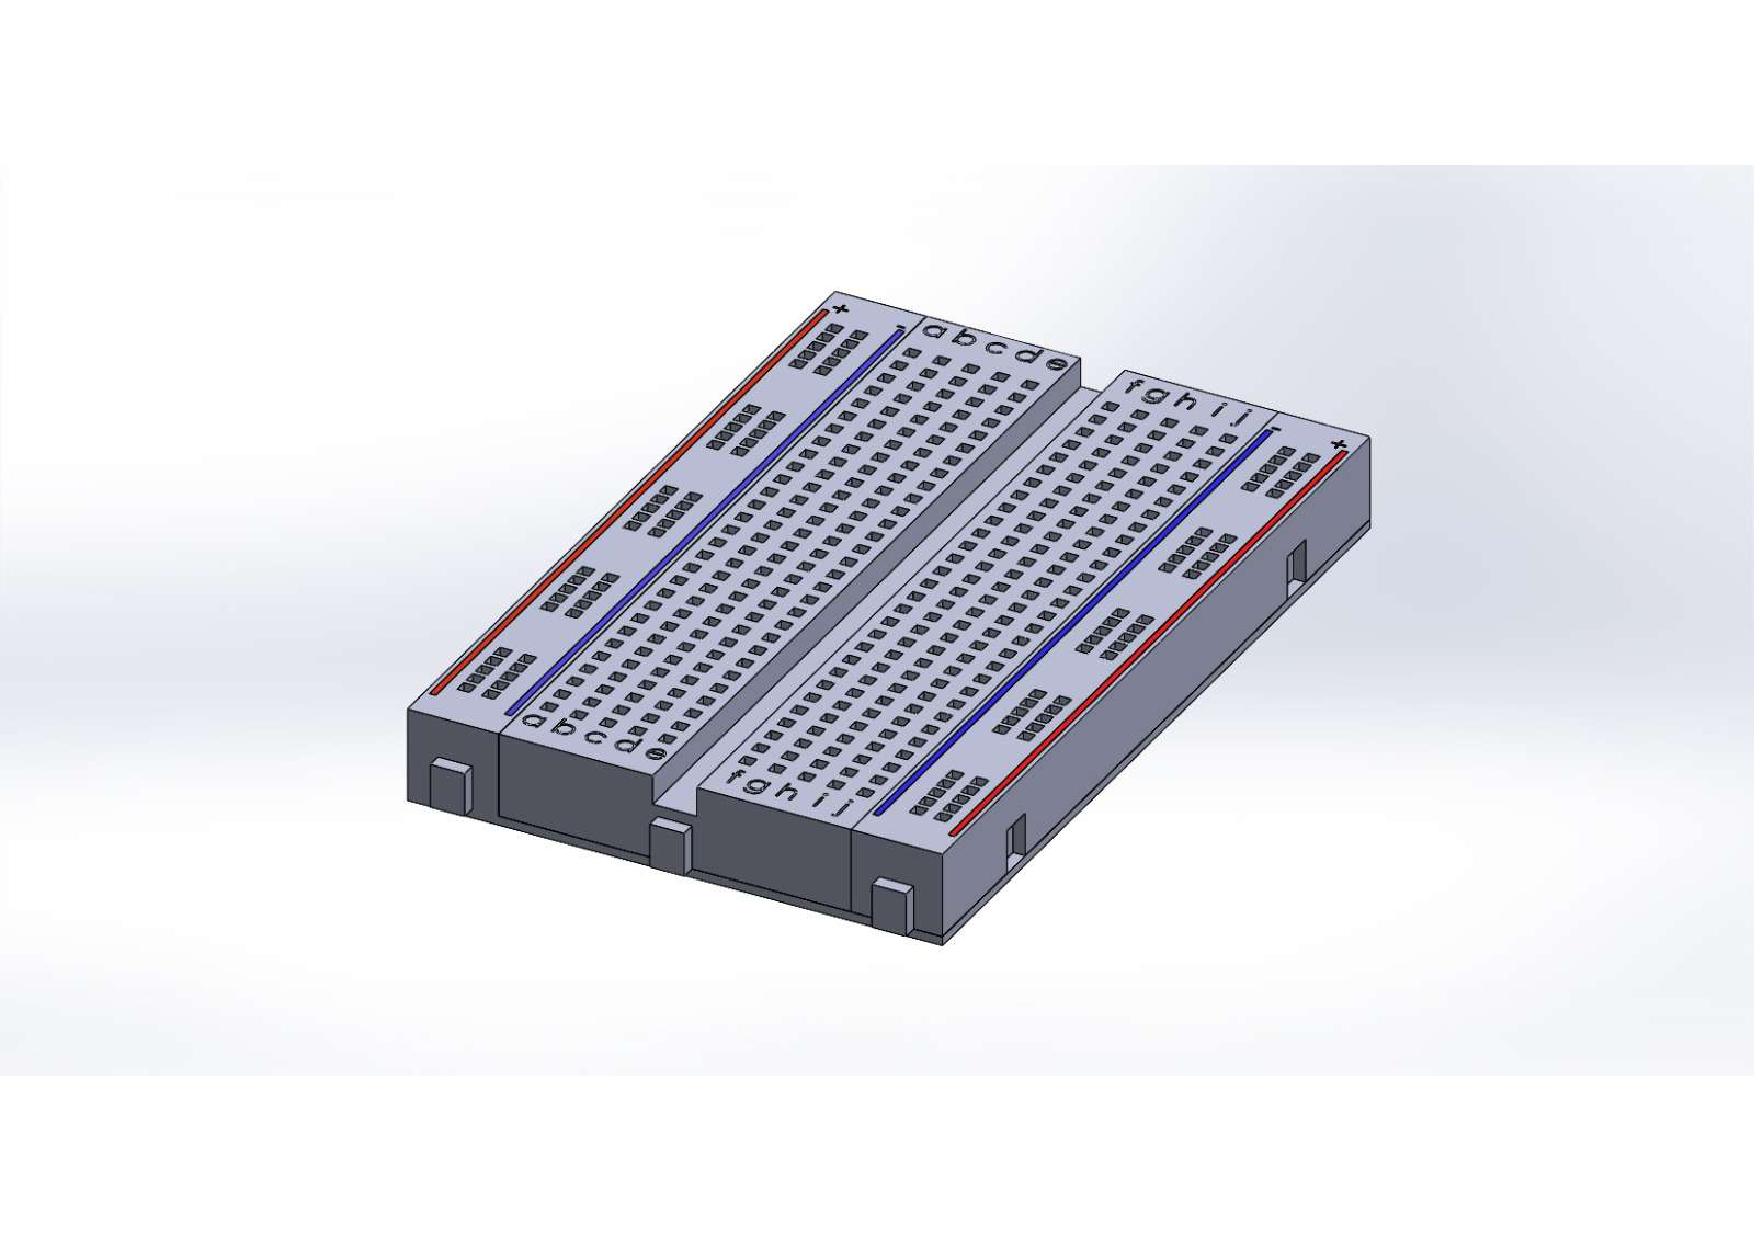
\includegraphics[trim = {65mm 40mm 65mm 40mm},clip,scale=0.5]{19/Img/protoboardFigura.pdf}
        \caption{Imagen del modelo 3D del Protoboard}
        \label{fig:protoboard}
    \end{figure}
    
    \item Resistencia: Pieza de plástico con alambre usada en los circuitos eléctricos como contra para la corriente eléctrica que pasa por ella, disminuyendo o forzando el cambio de dirección de esta corriente, esta se coloca dentro de los orificios del Protoboard para facilitar el flujo deseado de la corriente.\ref{fig:resistencia}.
    
            \begin{figure}[H]
        \centering
        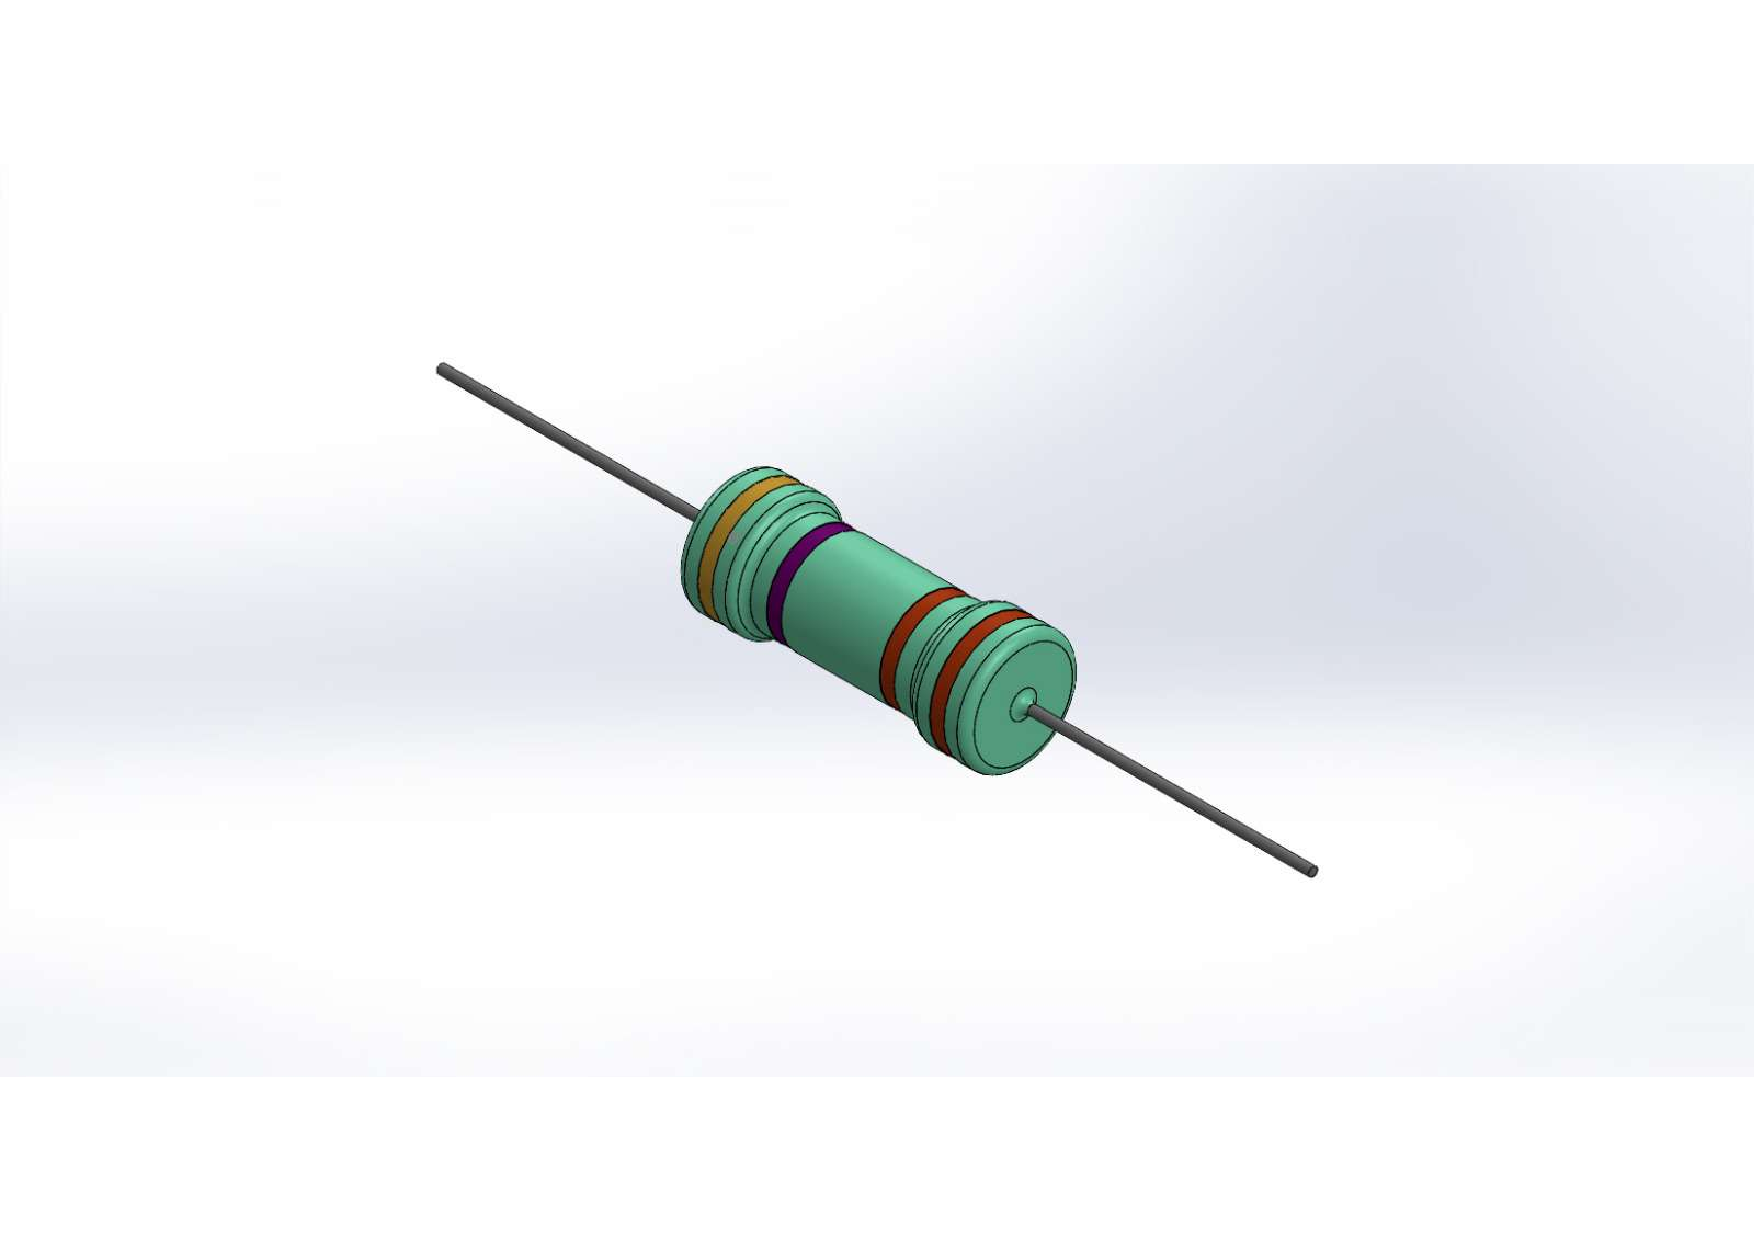
\includegraphics[trim = {65mm 40mm 80mm 60mm},clip,scale=0.5]{19/Img/resistenciaFigura.pdf}
        \caption{Imagen del modelo 3D de la resistencia}
        \label{fig:resistencia}
    \end{figure}
    
    \item Cable MM: Tipo de cable usado en la fabricación de circuitos eléctricos, este posee una varilla de metal por ambos lados lo cual permite el conectar dos elementos del tablero del Protoboard directamente.\ref{fig:cableMM}.
    
            \begin{figure}[H]
        \centering
        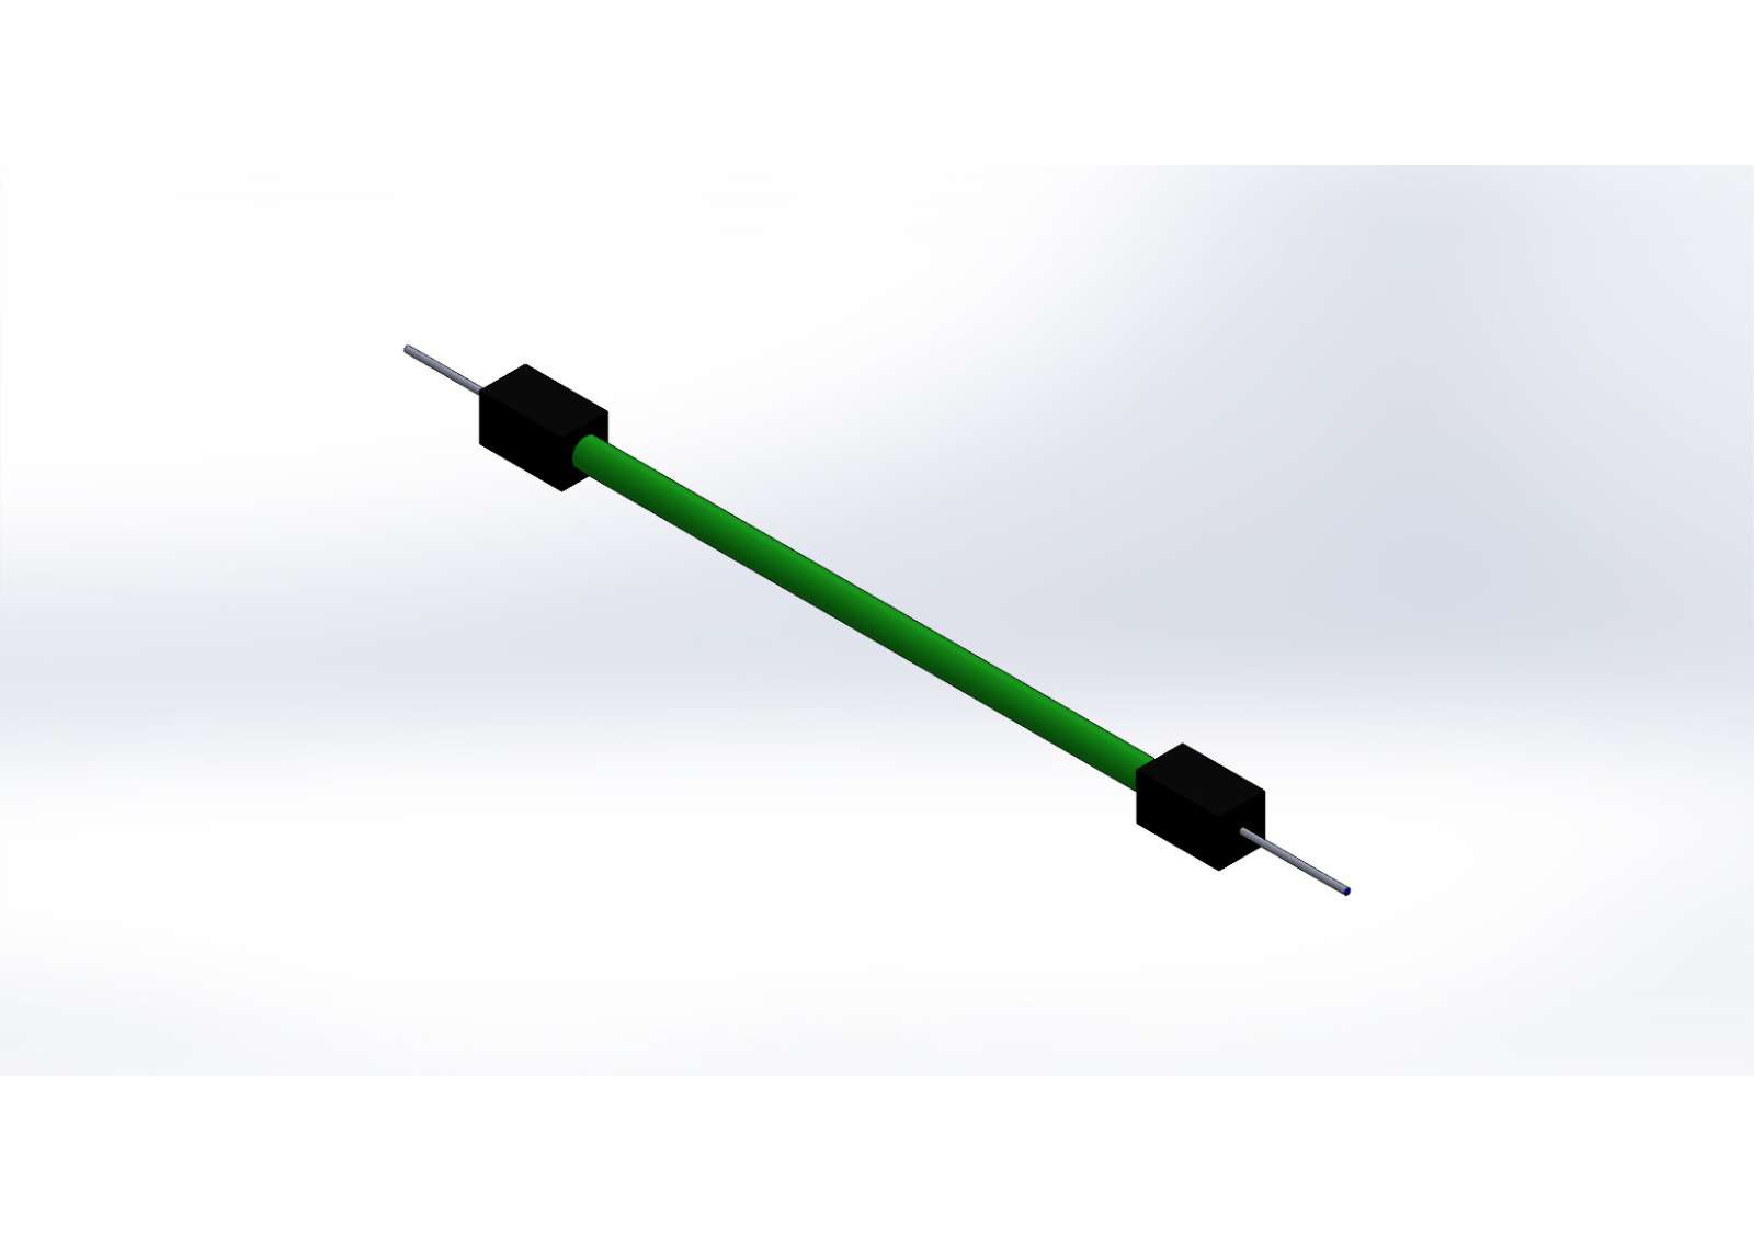
\includegraphics[trim = {70mm 60mm 60mm 50mm},clip,scale=0.5]{19/Img/cableMMFigura.pdf}
        \caption{Imagen del modelo 3D del cable MM}
        \label{fig:cableMM}
    \end{figure}
    
    \item Cable MH: Tipo de cable usado en la fabricación de circuitos eléctricos, este posee una varilla de metal solo por un lado del cable por lo cual este es usada comúnmente como extensión para que otro cable llegue a conectarse con otro que se encuentre a mayor distancia.\ref{fig:cableMH}.
    
            \begin{figure}[H]
        \centering
        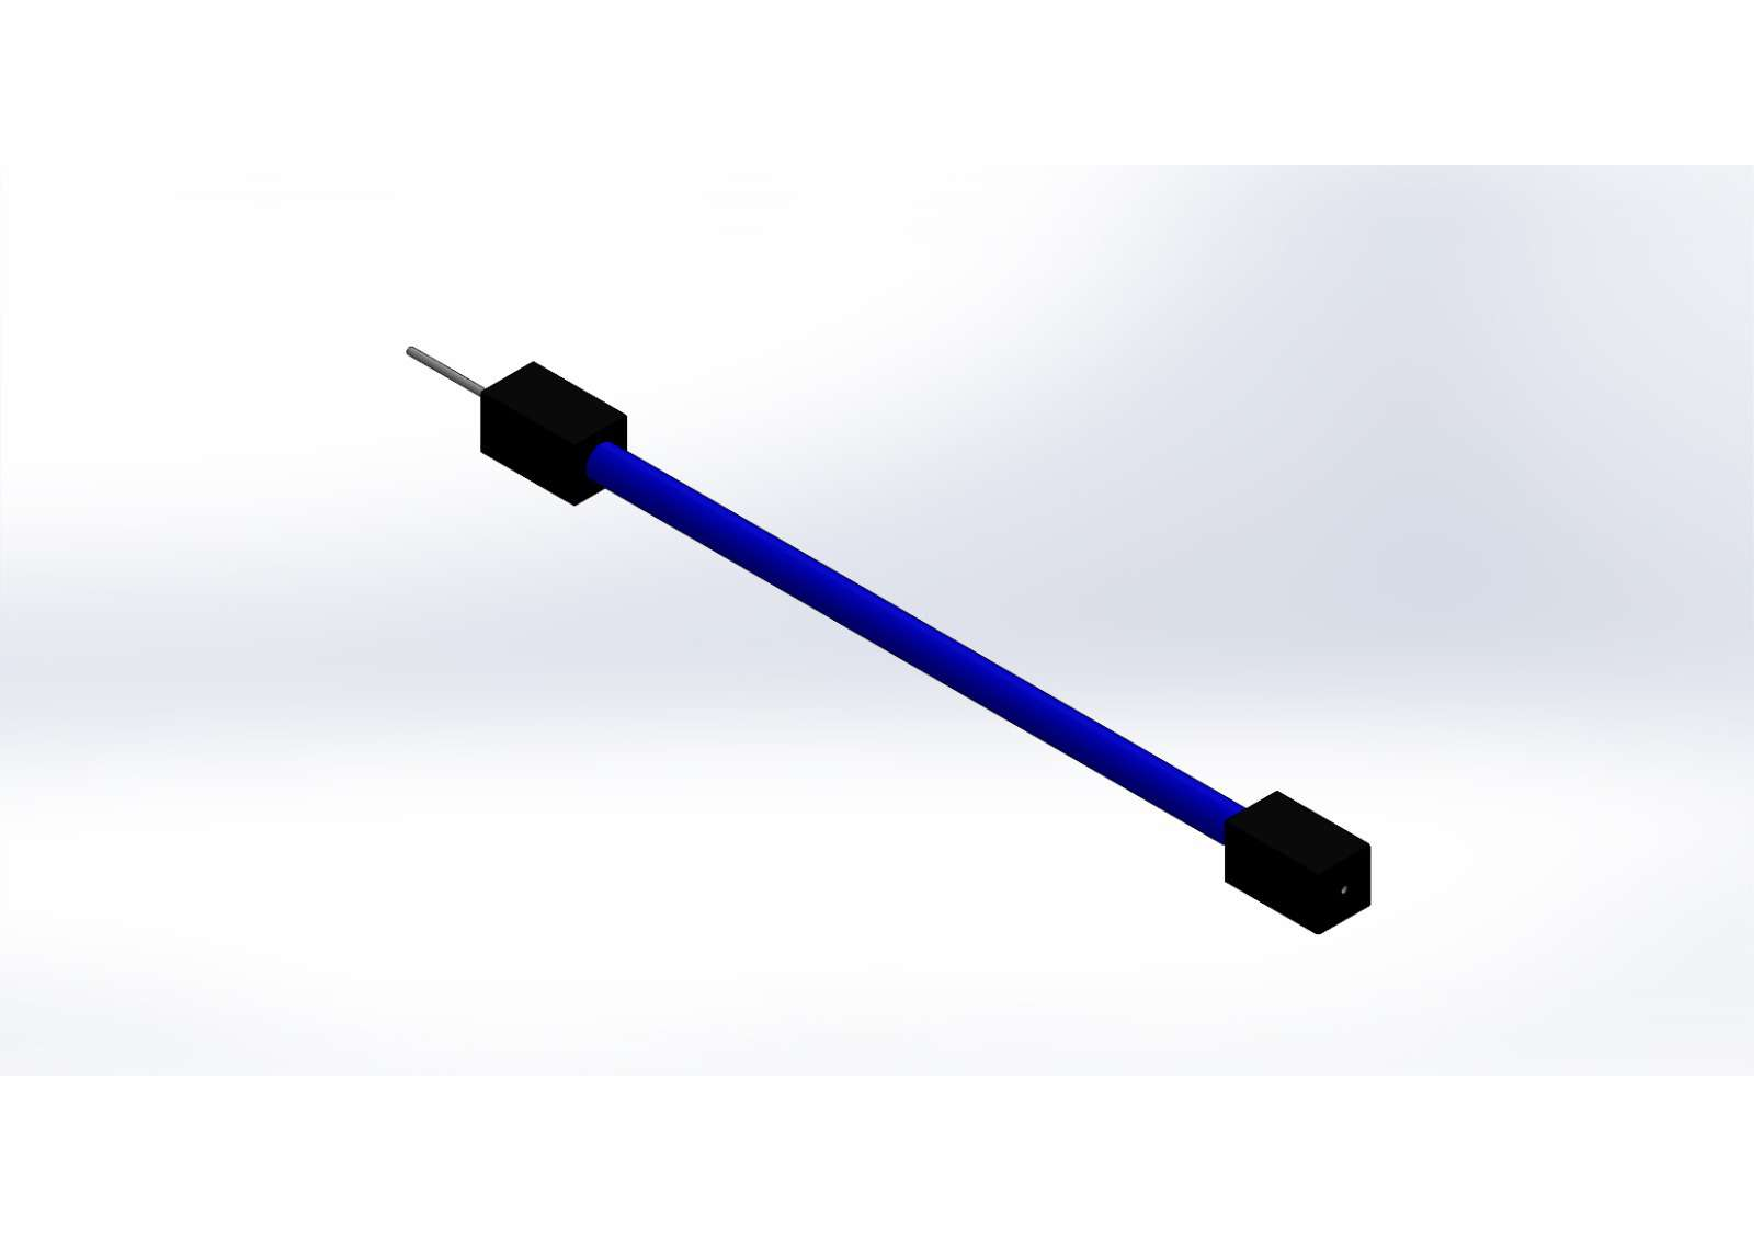
\includegraphics[trim = {65mm 30mm 60mm 40mm},clip,scale=0.5]{19/Img/cableMHFigura.pdf}
        \caption{Imagen del modelo 3D del cable MH}
        \label{fig:cableMH}
    \end{figure}
    
    \item Potenciómetro: Este posee el mismo funcionamiento que una resistencia, con la diferencia de que este puede variar, pudiendo modificar el valor de esta para colocarle el valor deseado, para mantener controlada la corriente total del circuito.\ref{fig:Potenciómetro}.
    
            \begin{figure}[H]
        \centering
        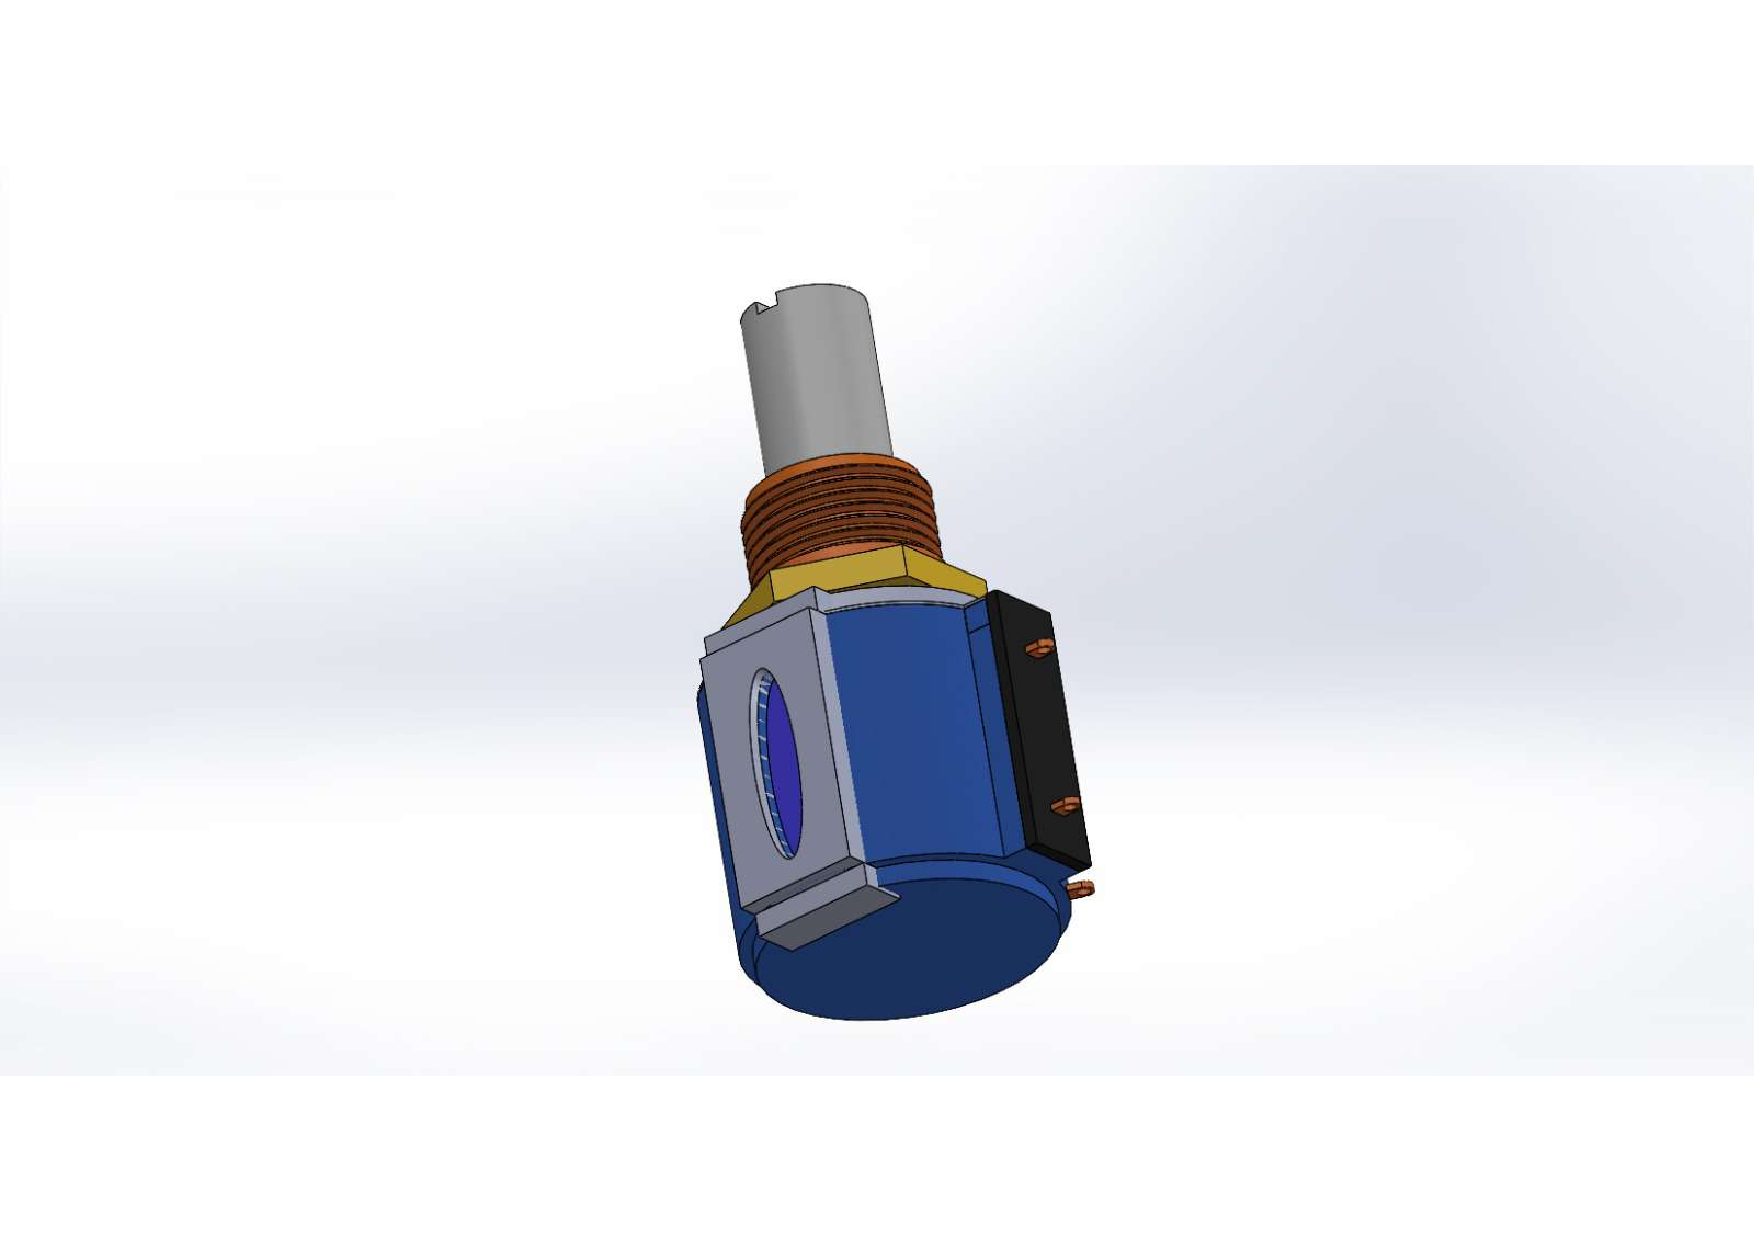
\includegraphics[trim = {65mm 30mm 60mm 40mm},clip,scale=0.5]{19/Img/potenciometroFigura.pdf}
        \caption{Imagen del modelo 3D del Potenciómetro}
        \label{fig:Potenciómetro}
    \end{figure}
        
    \item LCD: Pequeño dispositivo que posee una pantalla de cristal líquido, el cual es usado principalmente en los circuitos eléctricos para comprobar el funcionamiento de todas las piezas, mostrando mensajes que se programan con anterioridad dentro del circuito.\ref{fig:LCD}.
    
            \begin{figure}[H]
        \centering
        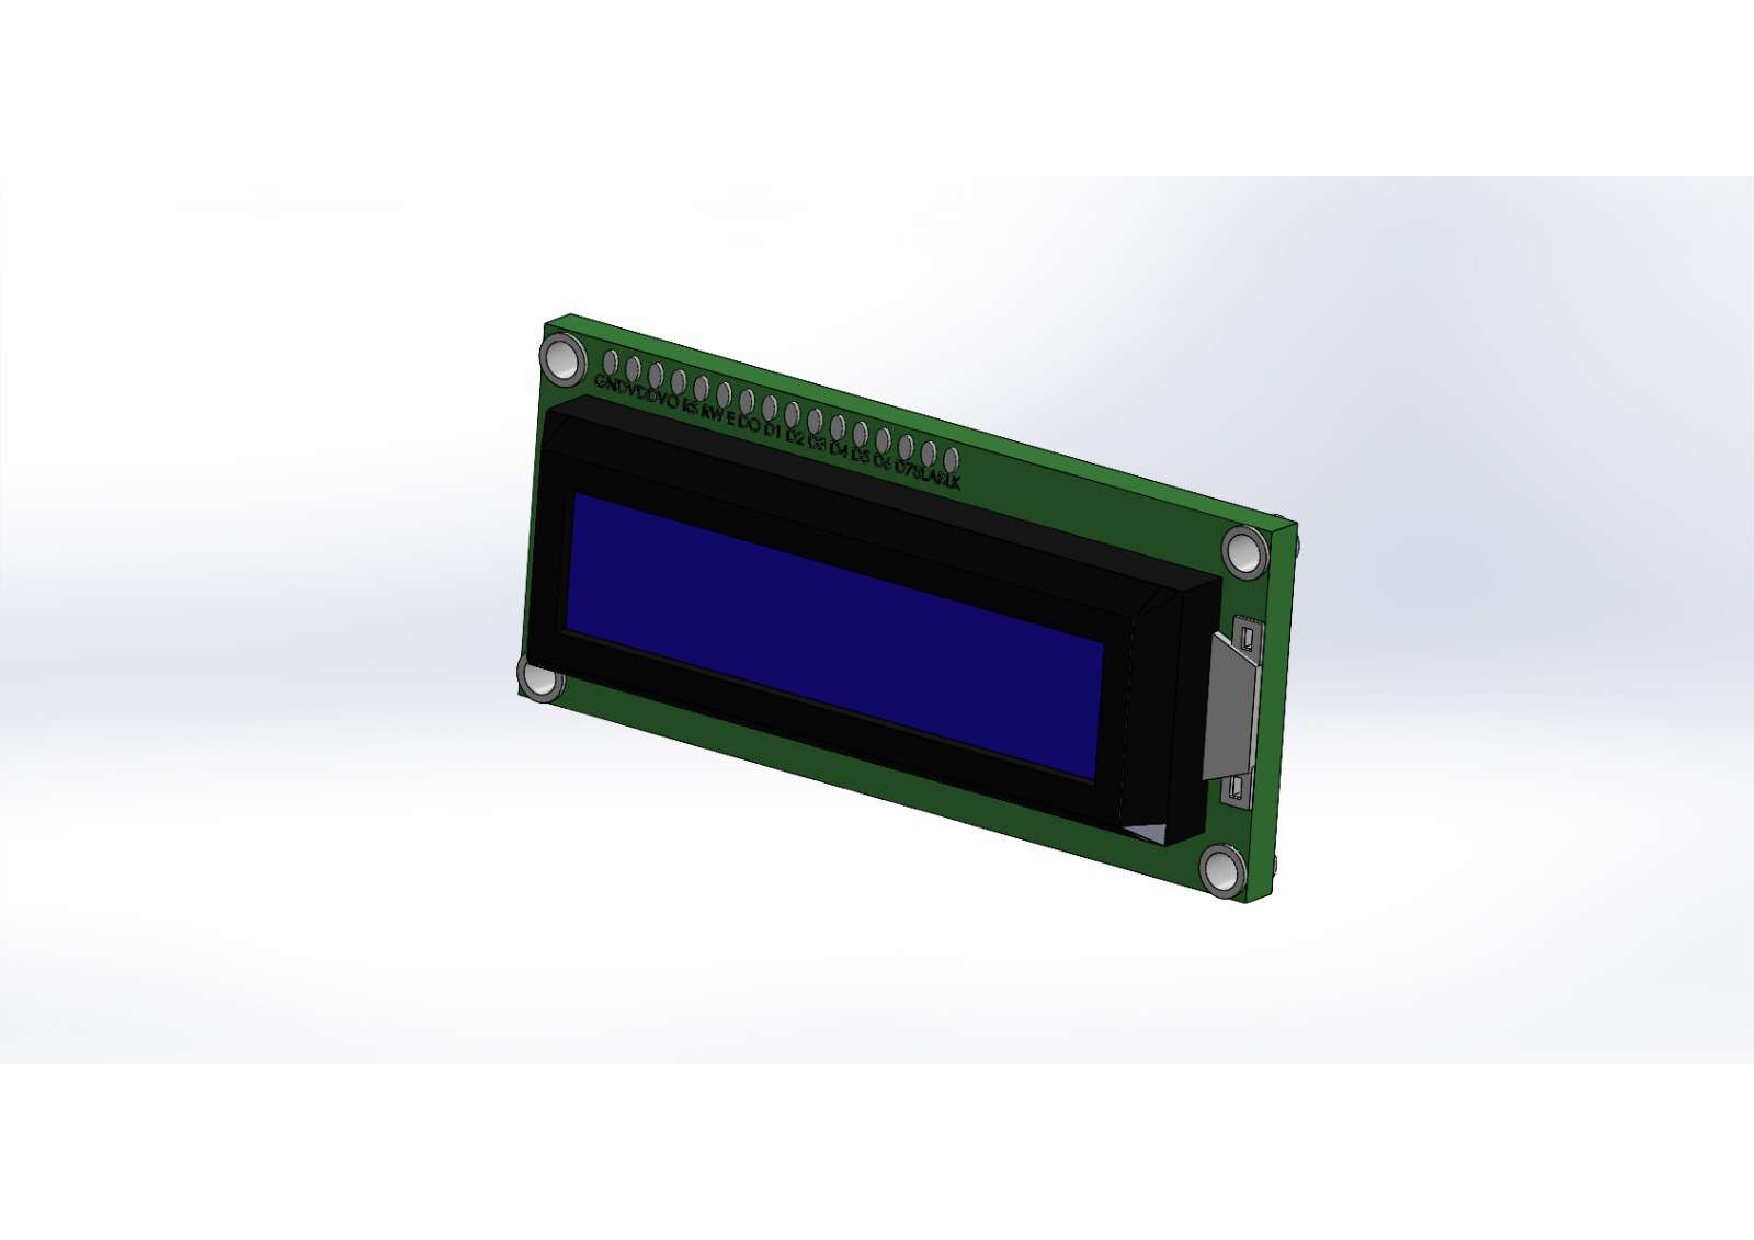
\includegraphics[trim = {65mm 60mm 60mm 50mm},clip,scale=0.5]{19/Img/icdFigura.pdf}
        \caption{Imagen del modelo 3D del LCD}
        \label{fig:LCD}
    \end{figure}
    
    \item Extensión: Objeto usado para expandir el cable conectado al circuito para que este pueda llegar a la fuente de energía.\ref{fig:Extension}.
    
            \begin{figure}[H]
        \centering
        \includegraphics[trim = {65mm 40mm 60mm 40mm},clip,scale=0.5]{19/Img/extensiónFigura.pdf}
        \caption{Imagen del modelo 3D de la Extensión}
        \label{fig:Extension}
    \end{figure}
    
    \item Cable USB: Cable usado para darle una fuente de energía directa al circuito eléctrico, este posee dos conexiones iguales saliendo de ambos lados del cable.\ref{fig:CableUSB}.
    
            \begin{figure}[H]
        \centering
        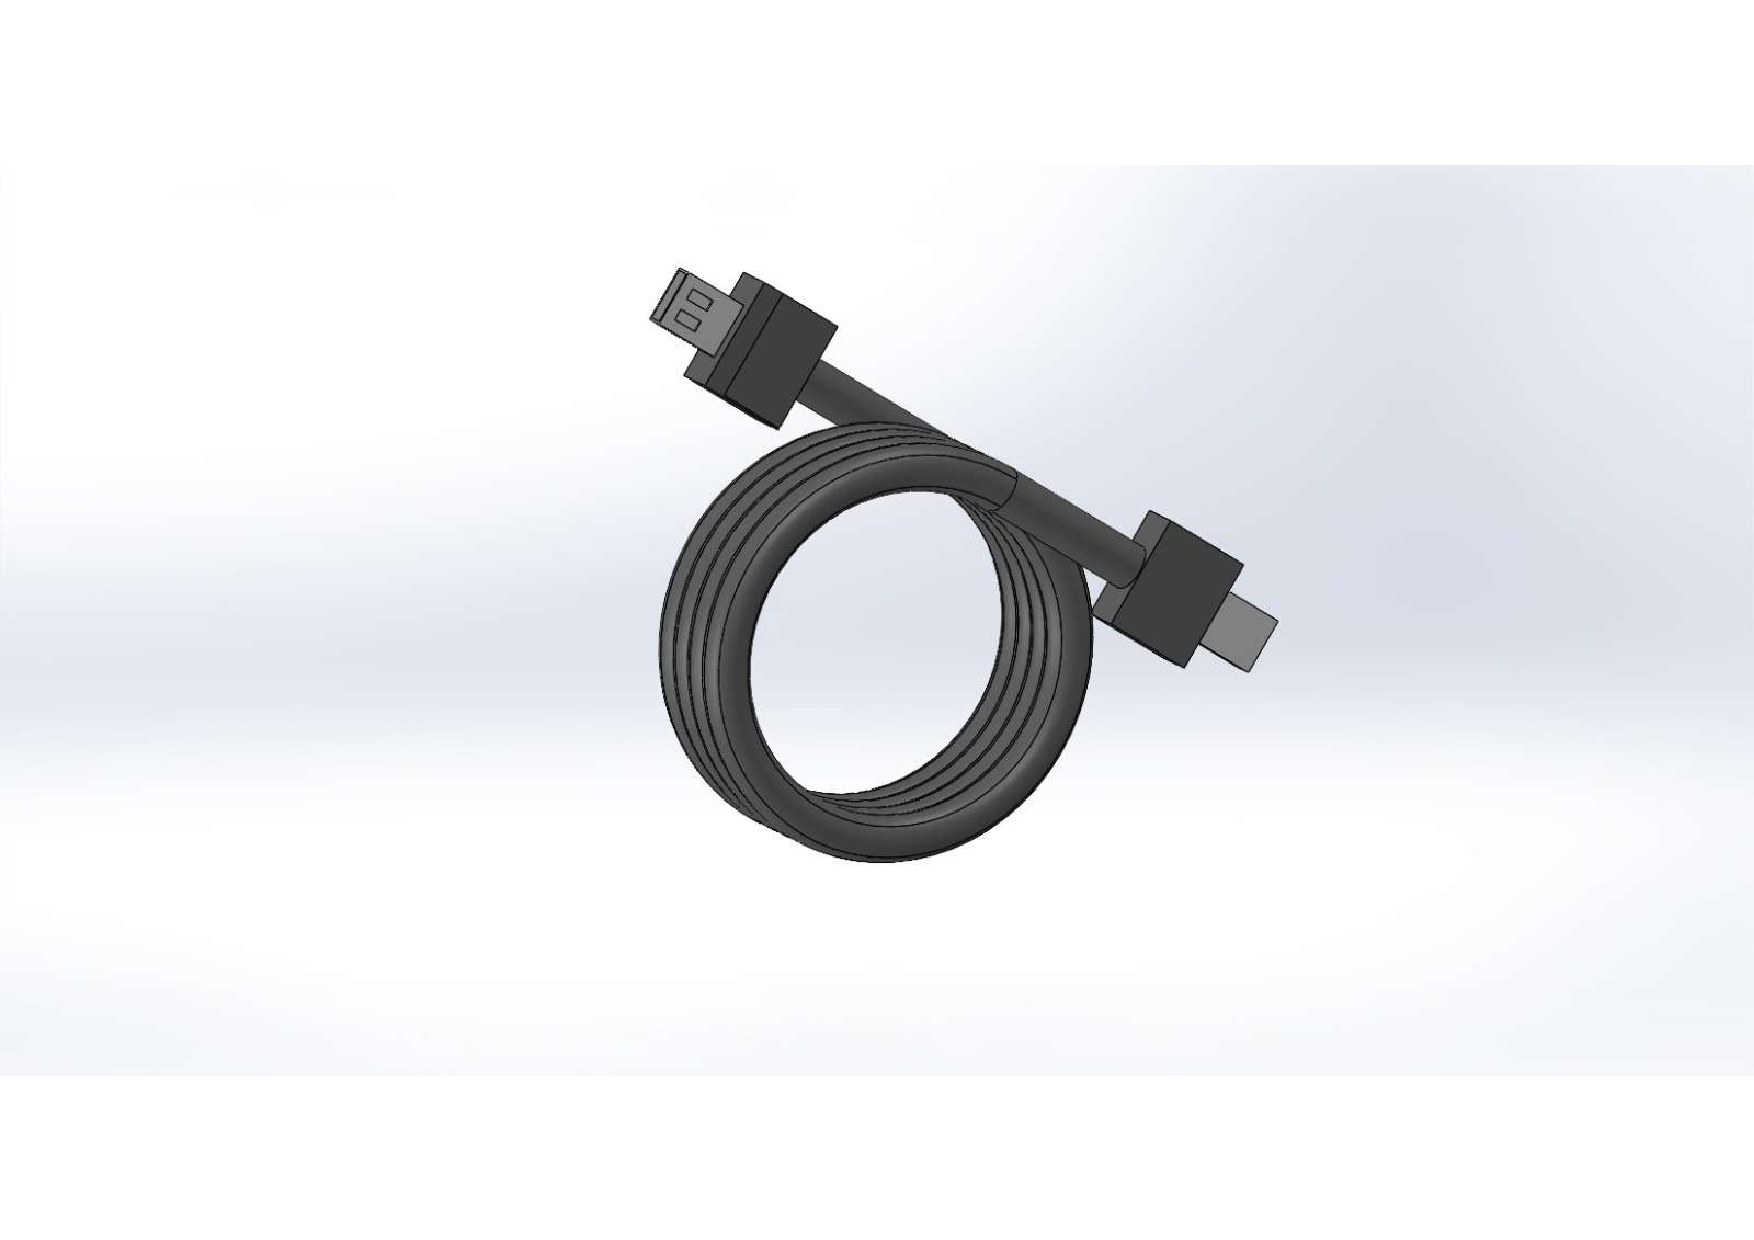
\includegraphics[trim = {65mm 40mm 60mm 40mm},clip,scale=0.5]{19/Img/cableUSBFigura.pdf}
        \caption{Imagen del modelo 3D del cable USB}
        \label{fig:CableUSB}
    \end{figure}
    
    \item ESP-32: Este chip es un microcontrolador soldado directamente al Protoboard, el cual permite poseer tanto un receptor como un emisor de señal saliente del Protoboard.\ref{fig:ESP-32}.
    
            \begin{figure}[H]
        \centering
        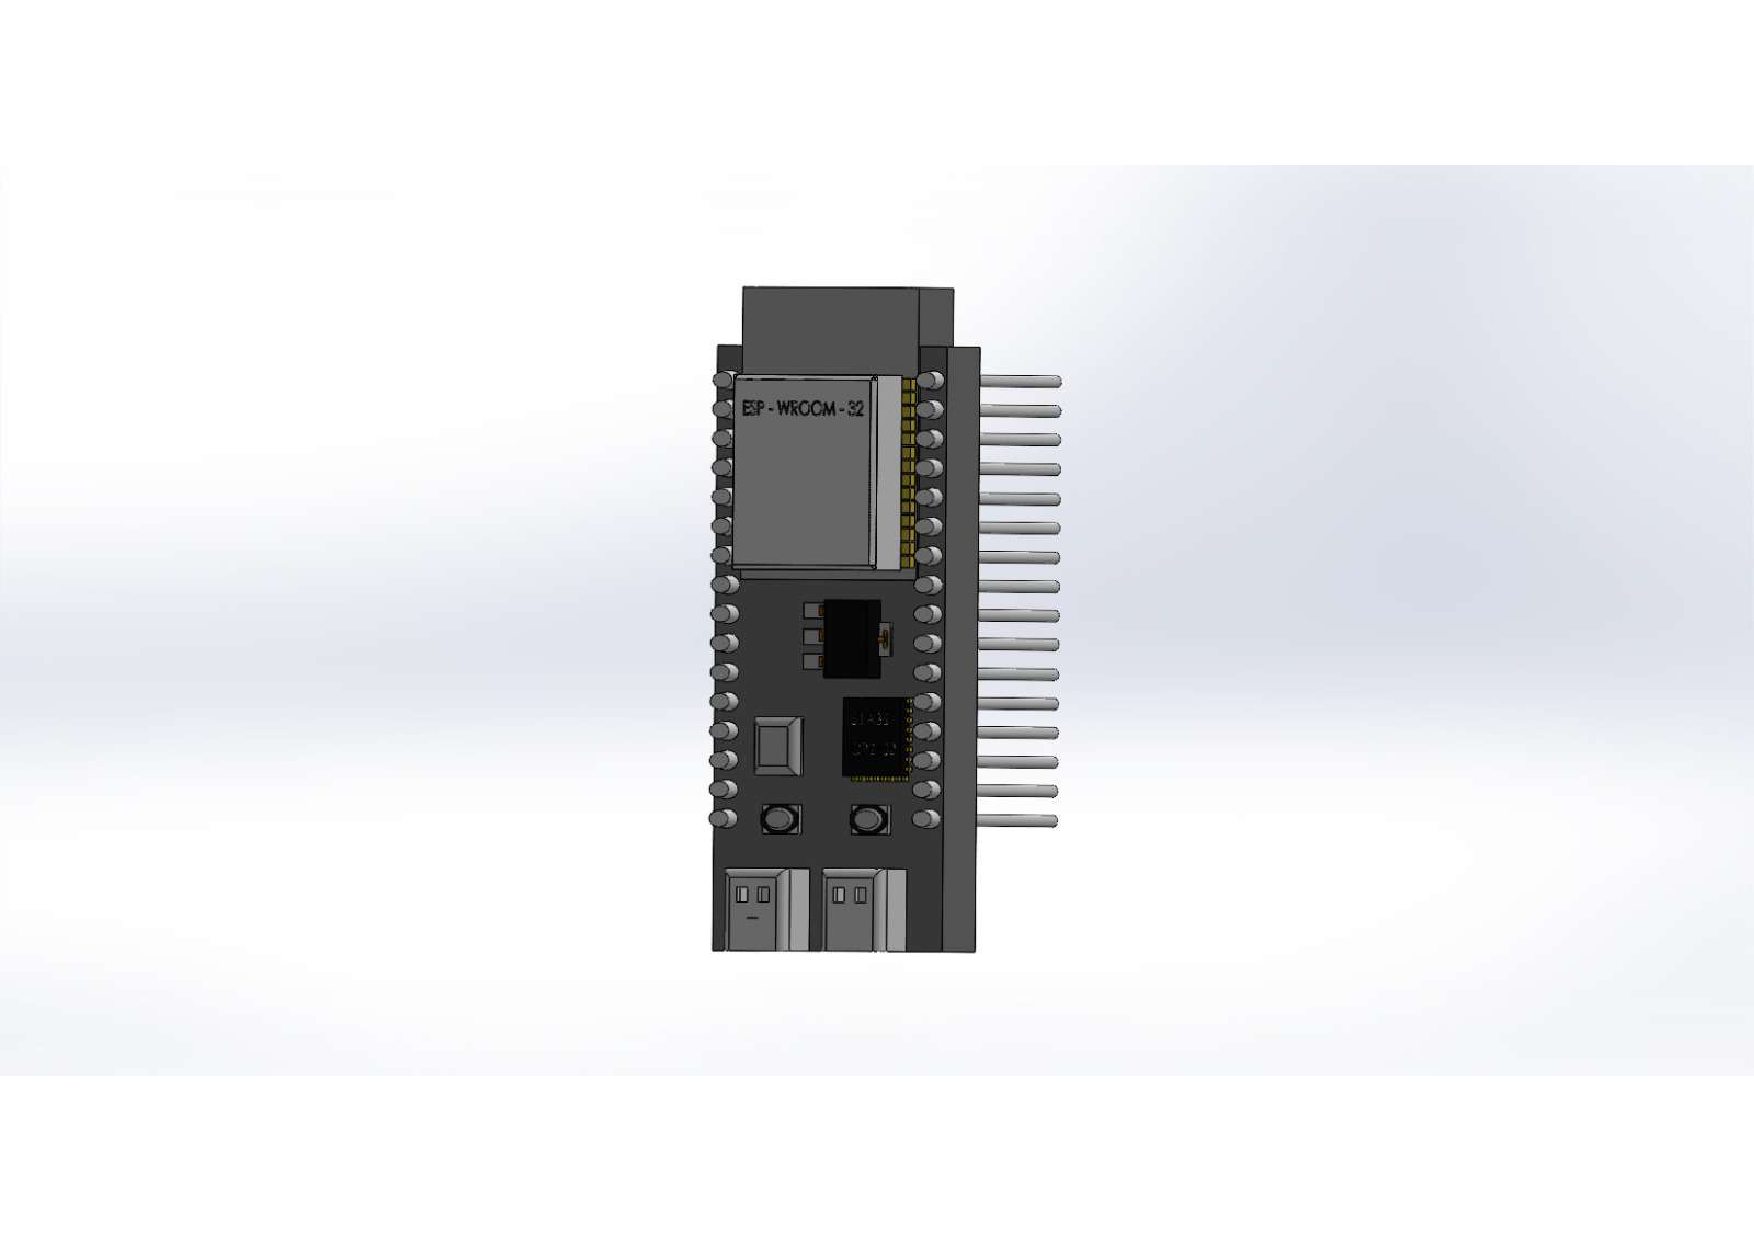
\includegraphics[trim = {65mm 35mm 60mm 40mm},clip,scale=0.5]{19/Img/esp-32Figura.pdf}
        \caption{Imagen del modelo 3D del ESP-32}
        \label{fig:ESP-32}
    \end{figure}
    
    \item Módulo I2C Interfaz: Este es un modulo de interfaz que permite facilitar el manejo y utilización de las pantallas, siendo soldada en la parte posterior de la LCD para su uso en el circuito.\ref{fig:modulo}.
    
            \begin{figure}[H]
        \centering
        \includegraphics[trim = {65mm 35mm 60mm 40mm},clip,scale=0.5]{19/Img/móduloI2CInterfazFigura.pdf}
        \caption{Imagen del modelo 3D del Módulo I2C Interfaz}
        \label{fig:modulo}
    \end{figure}
        \end{itemize}
    
              \newpage
    
    \newpage
    A continuación presentare una lista de dibujos de las piezas a utilizar con el propósito de ofrecer las medidas base que se emplearan de cada material a la hora de realizar el ensamble del circuito presentado en este proceso:
                \newpage
                \begin{figure}[H]
        \centering
        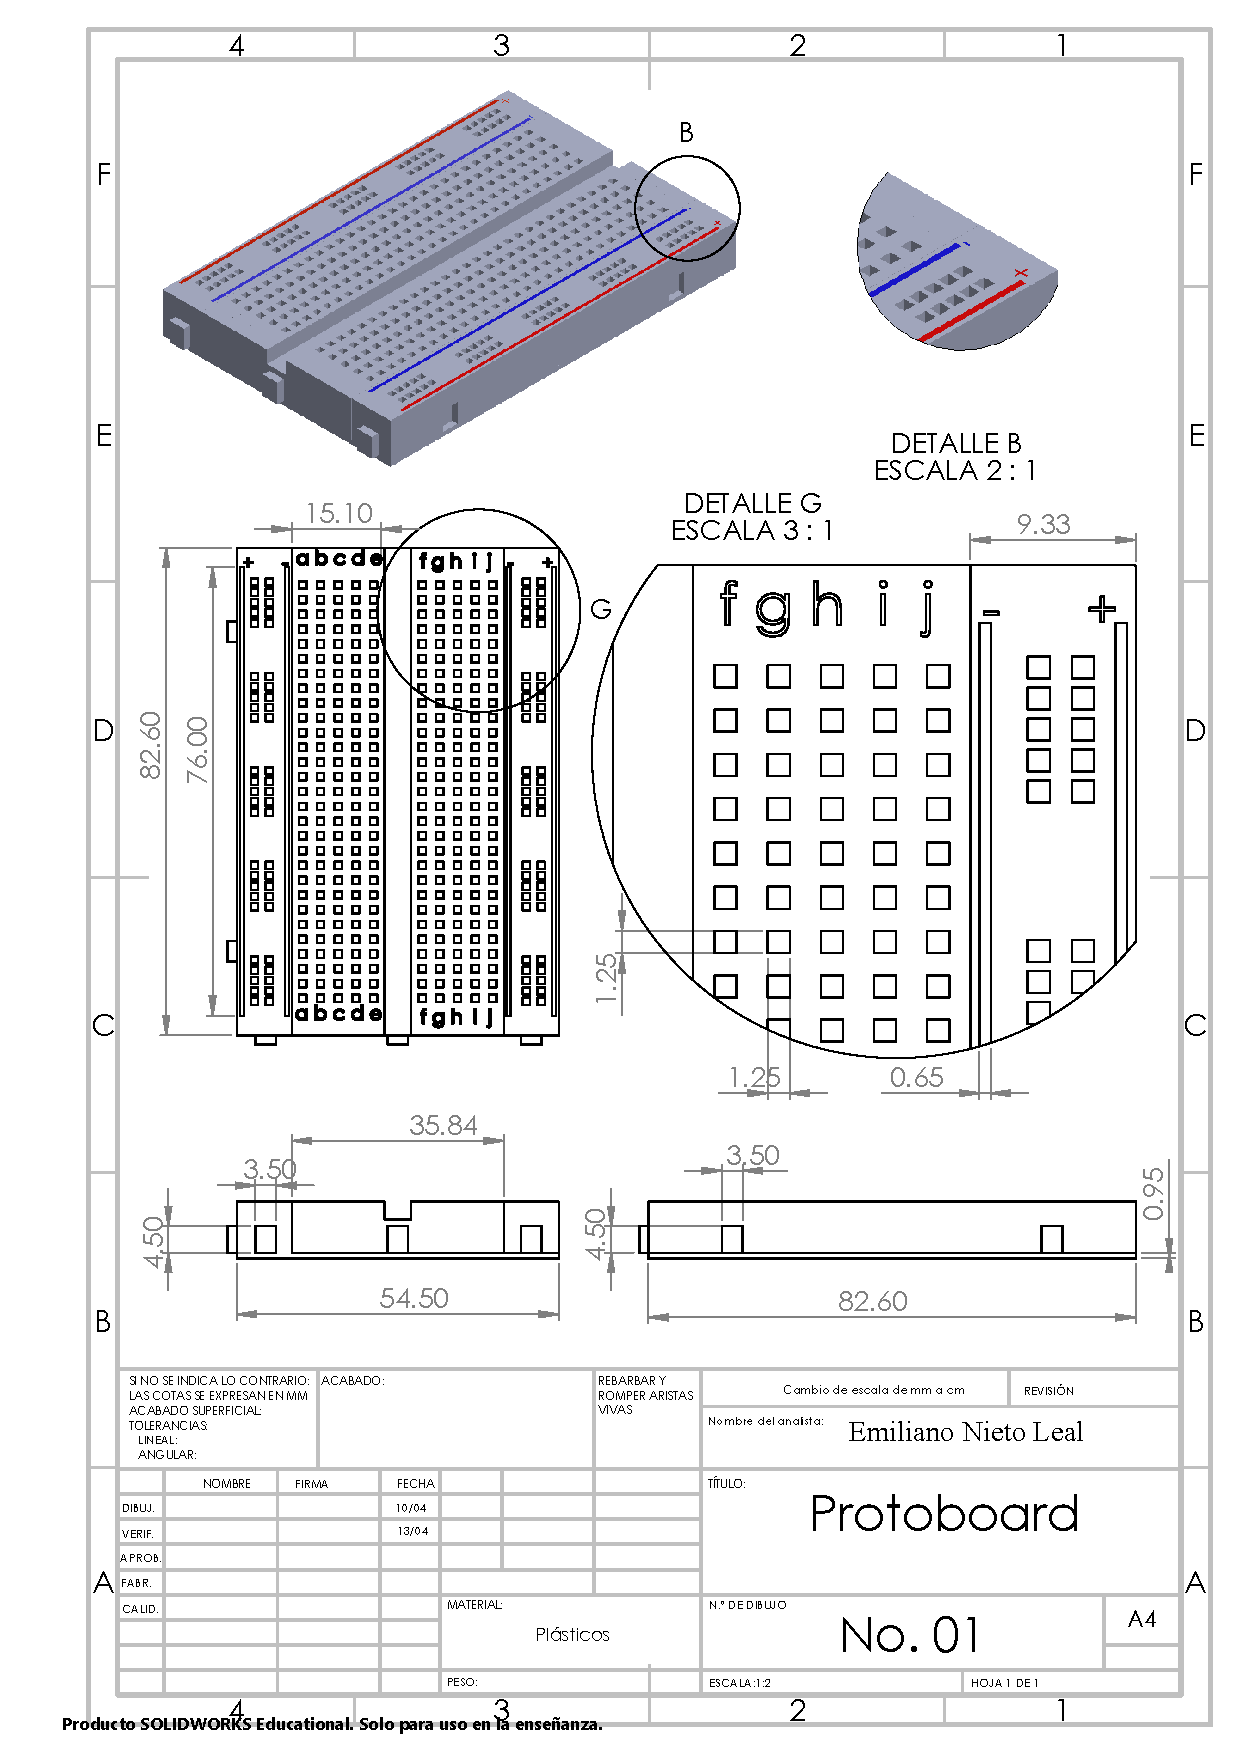
\includegraphics[trim = {1mm 1mm 1mm 1mm},clip,scale=0.5]{19/Img/protoboardDibujo.pdf}
        \caption{Dibujo Protoboard}
        \label{fig:Dibujo Protoboard}
    \end{figure}
        
    
    \newpage
                \begin{figure}[H]
        \centering
        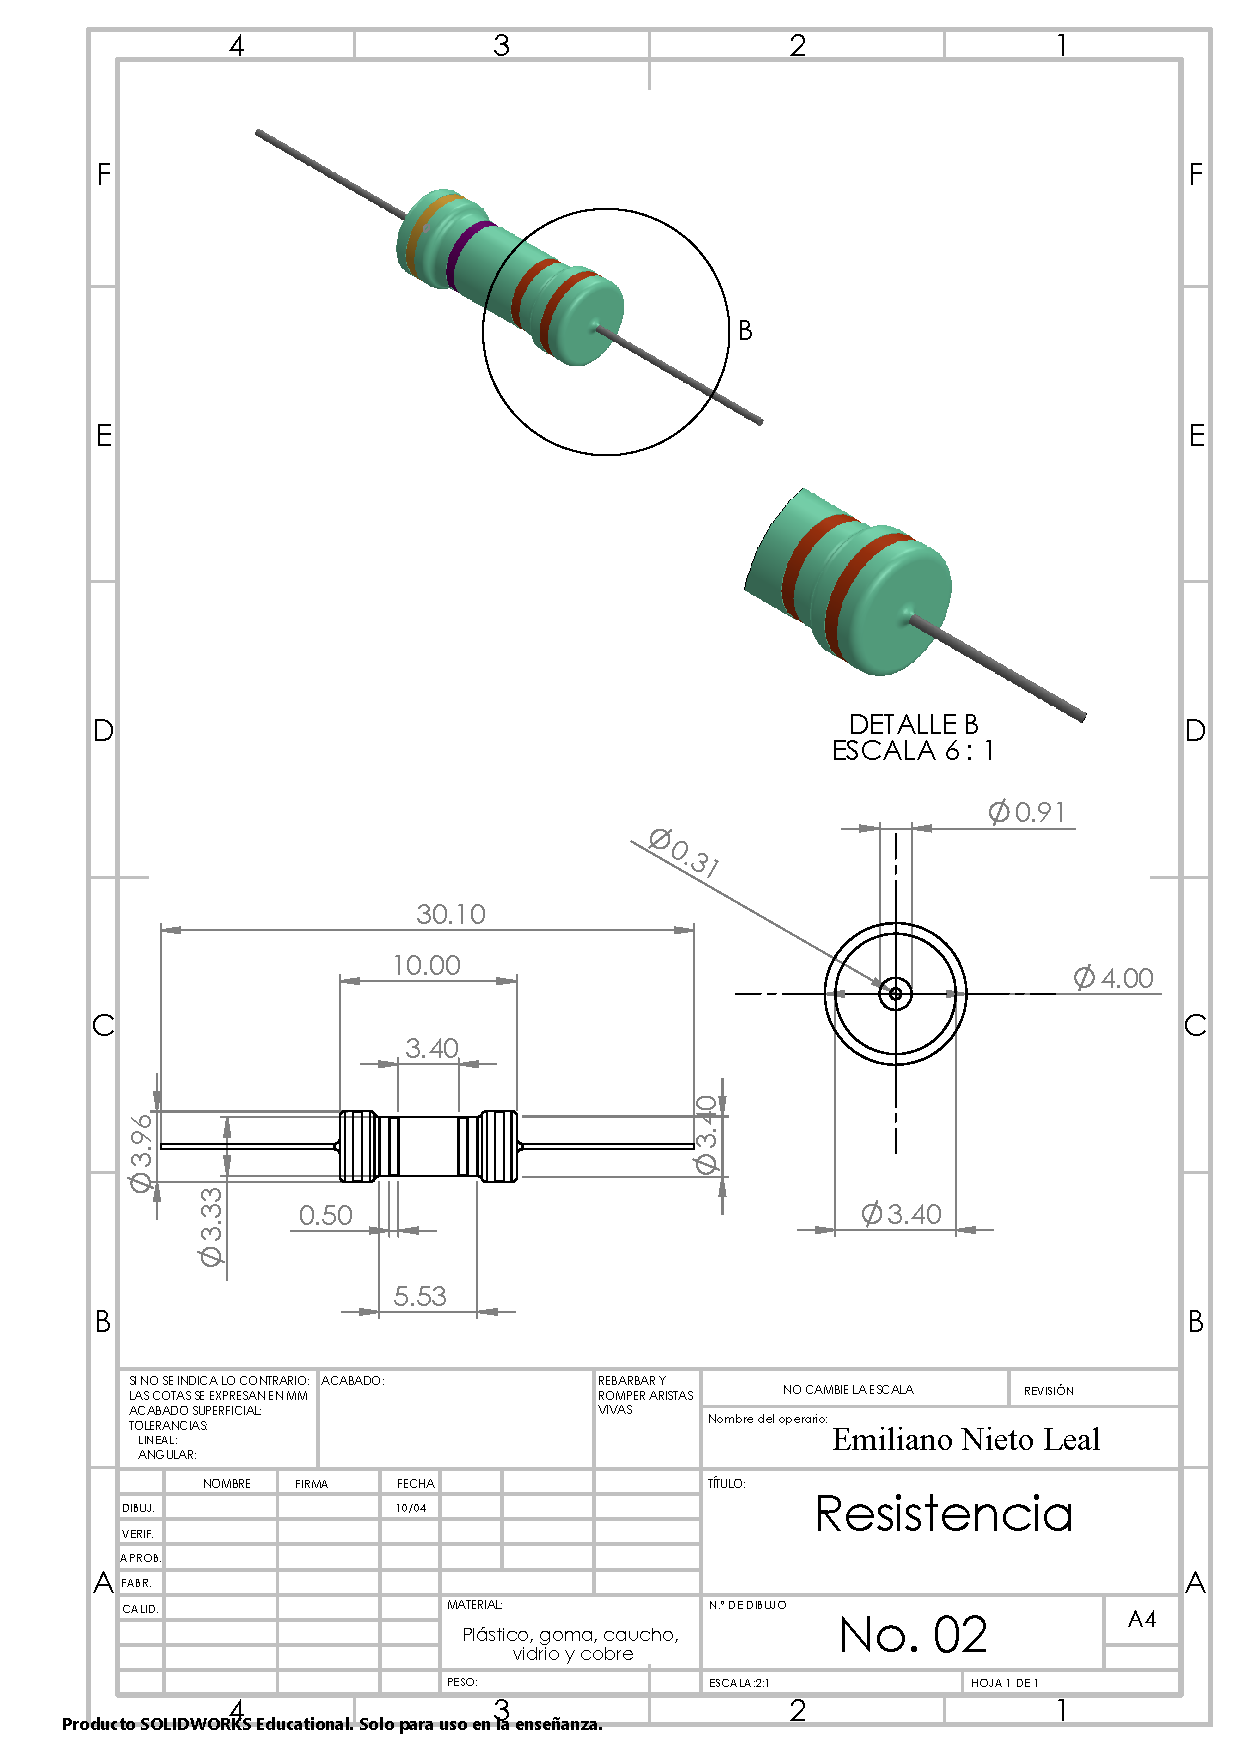
\includegraphics[trim = {1mm 1mm 1mm 1mm},clip,scale=0.5]{19/Img/resistenciaDibujo.pdf}
        \caption{Dibujo resistencia}
        \label{fig:Dibujo resistencia}
    \end{figure}
        
    \newpage
                \begin{figure}[H]
        \centering
        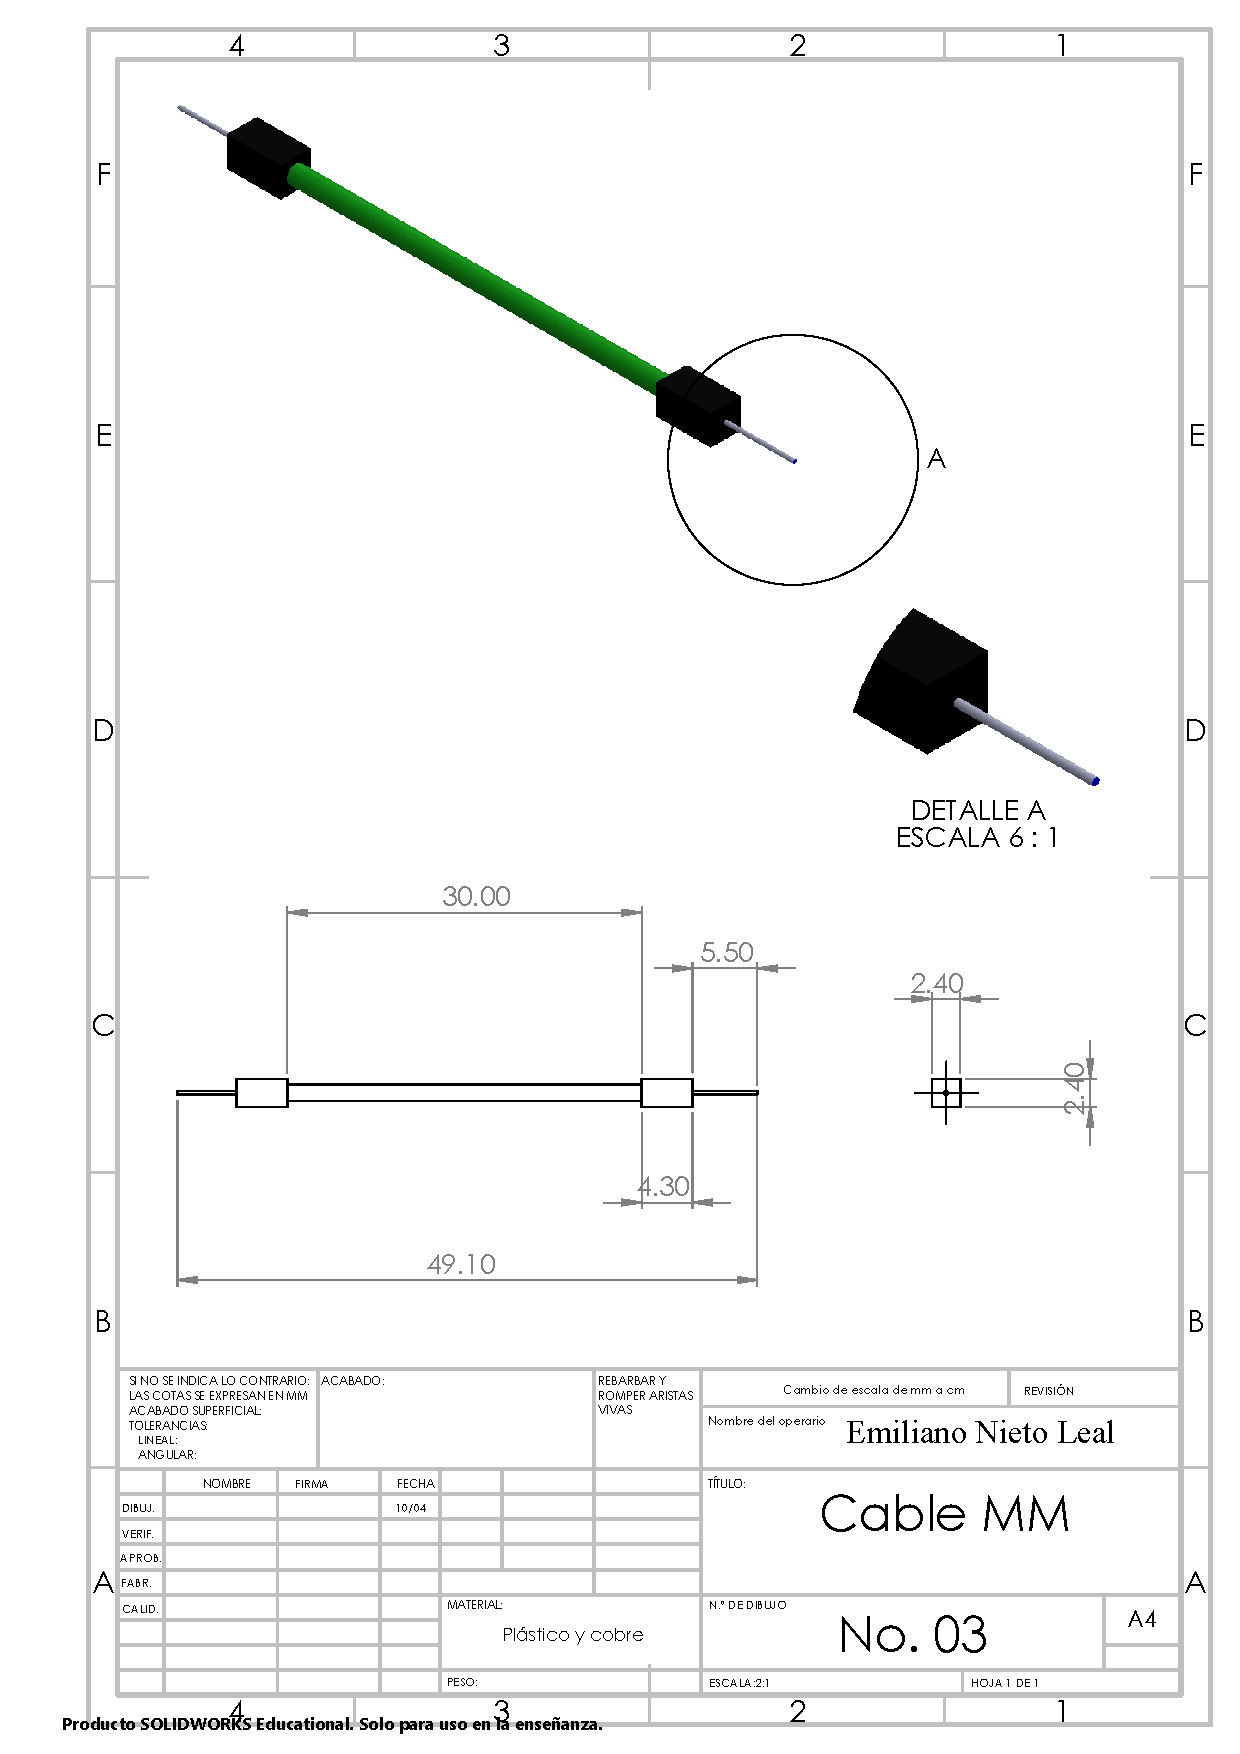
\includegraphics[trim = {1mm 1mm 1mm 1mm},clip,scale=0.5]{19/Img/cableMMDibujo.pdf}
        \caption{Dibujo CableMM}
        \label{fig:Dibujo cableMM}
    \end{figure}
        \newpage
                \begin{figure}[H]
        \centering
        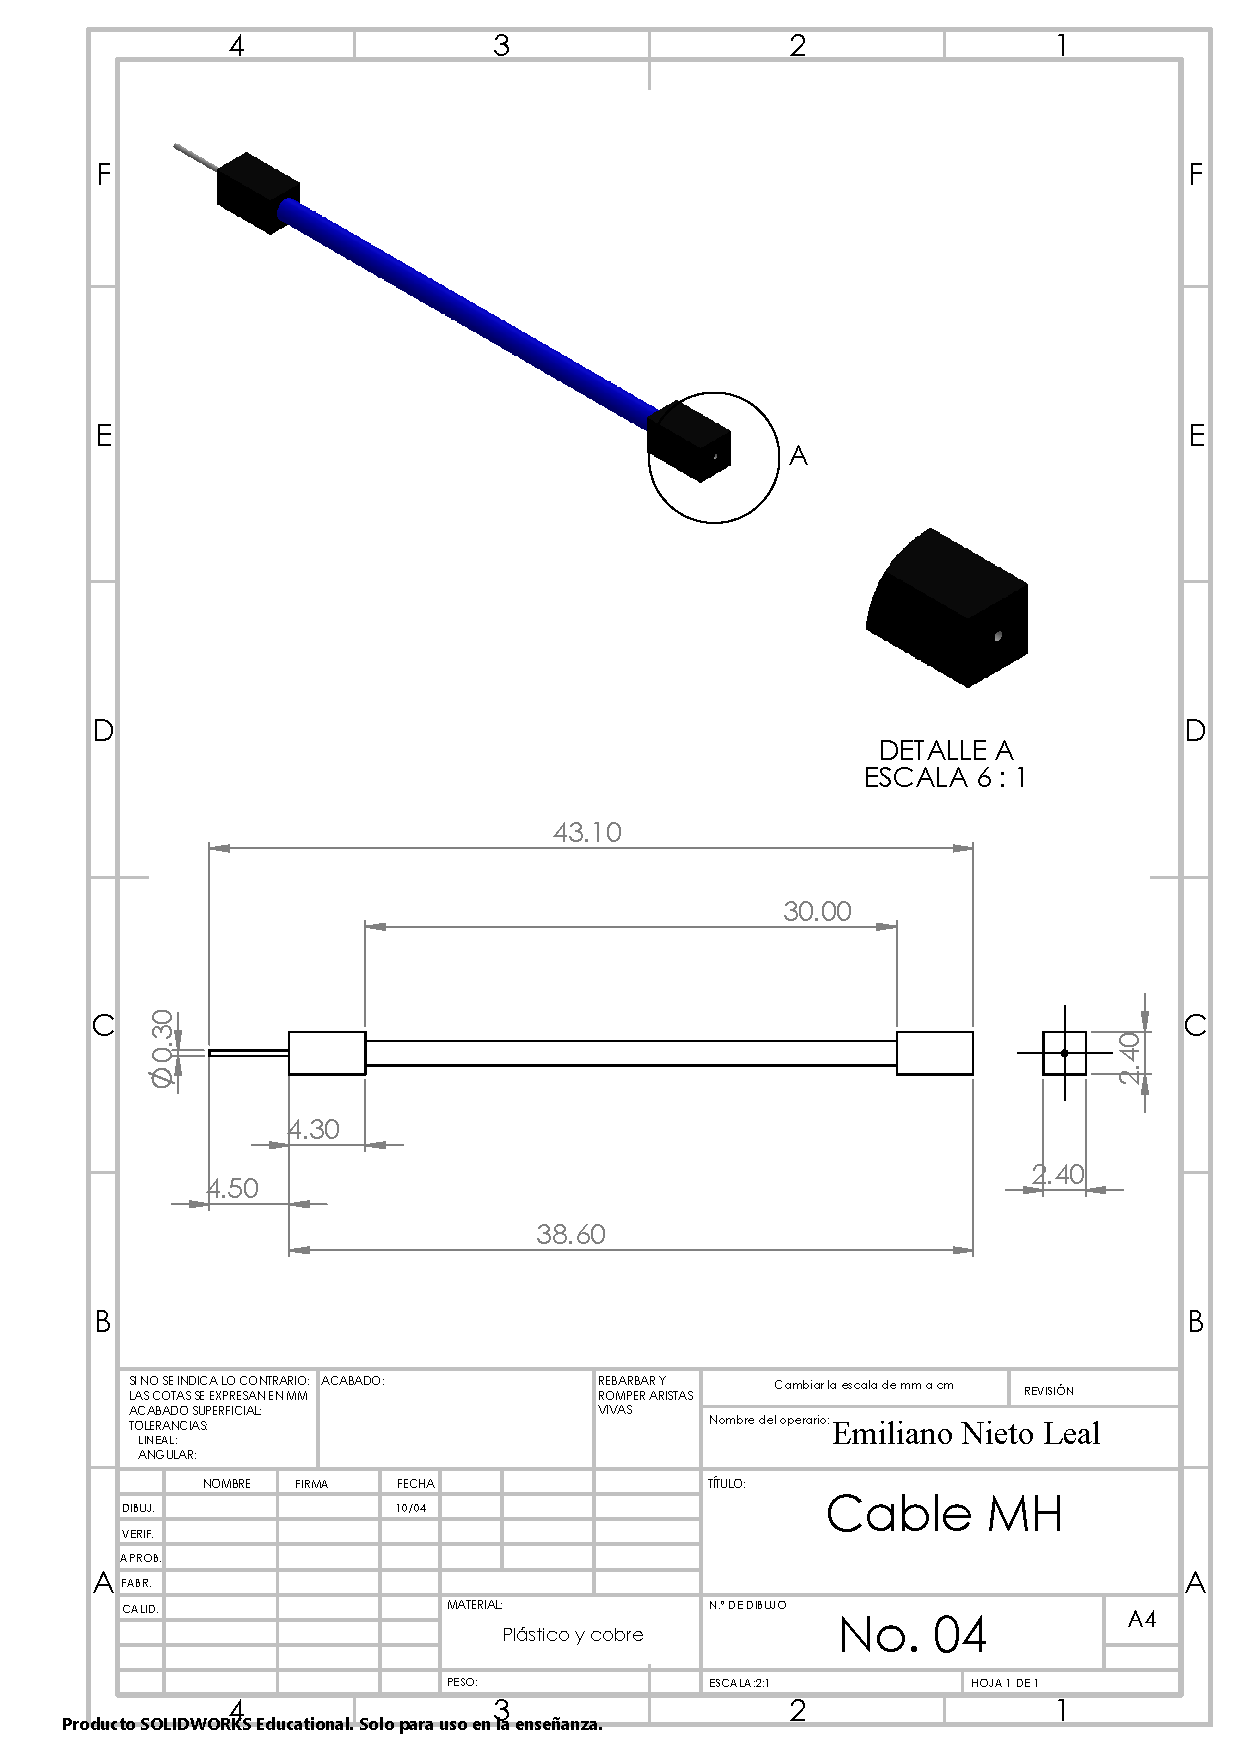
\includegraphics[trim = {1mm 1mm 1mm 1mm},clip,scale=0.5]{19/Img/cableMHDibujo.pdf}
        \caption{Dibujo CableMH}
        \label{fig:Dibujo cableMH}
    \end{figure}
            \newpage
                \begin{figure}[H]
        \centering
        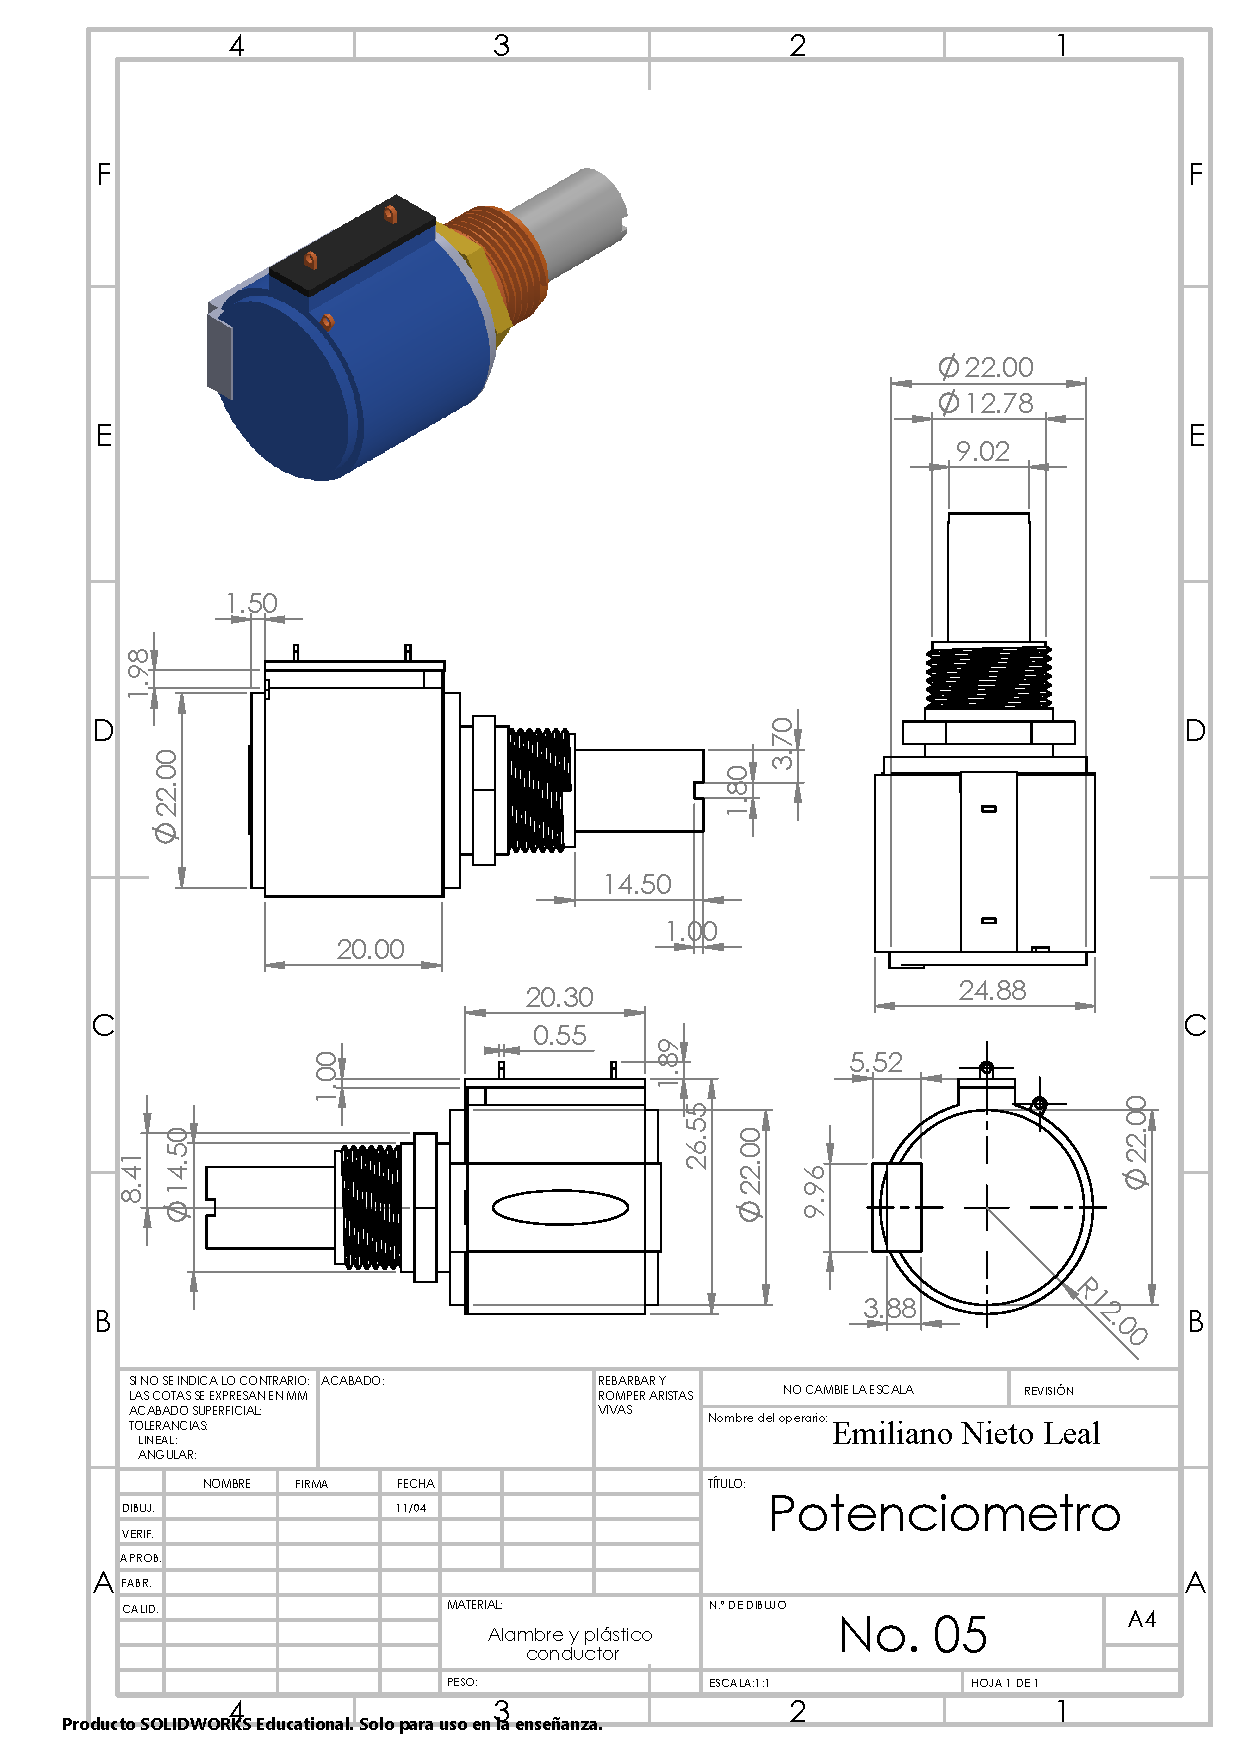
\includegraphics[trim = {1mm 1mm 1mm 1mm},clip,scale=0.5]{19/Img/potenciometroDibujo.pdf}
        \caption{Dibujo Potenciómetro}
        \label{fig:Dibujo Potenciómetro}
    \end{figure}
                \newpage
                \begin{figure}[H]
        \centering
        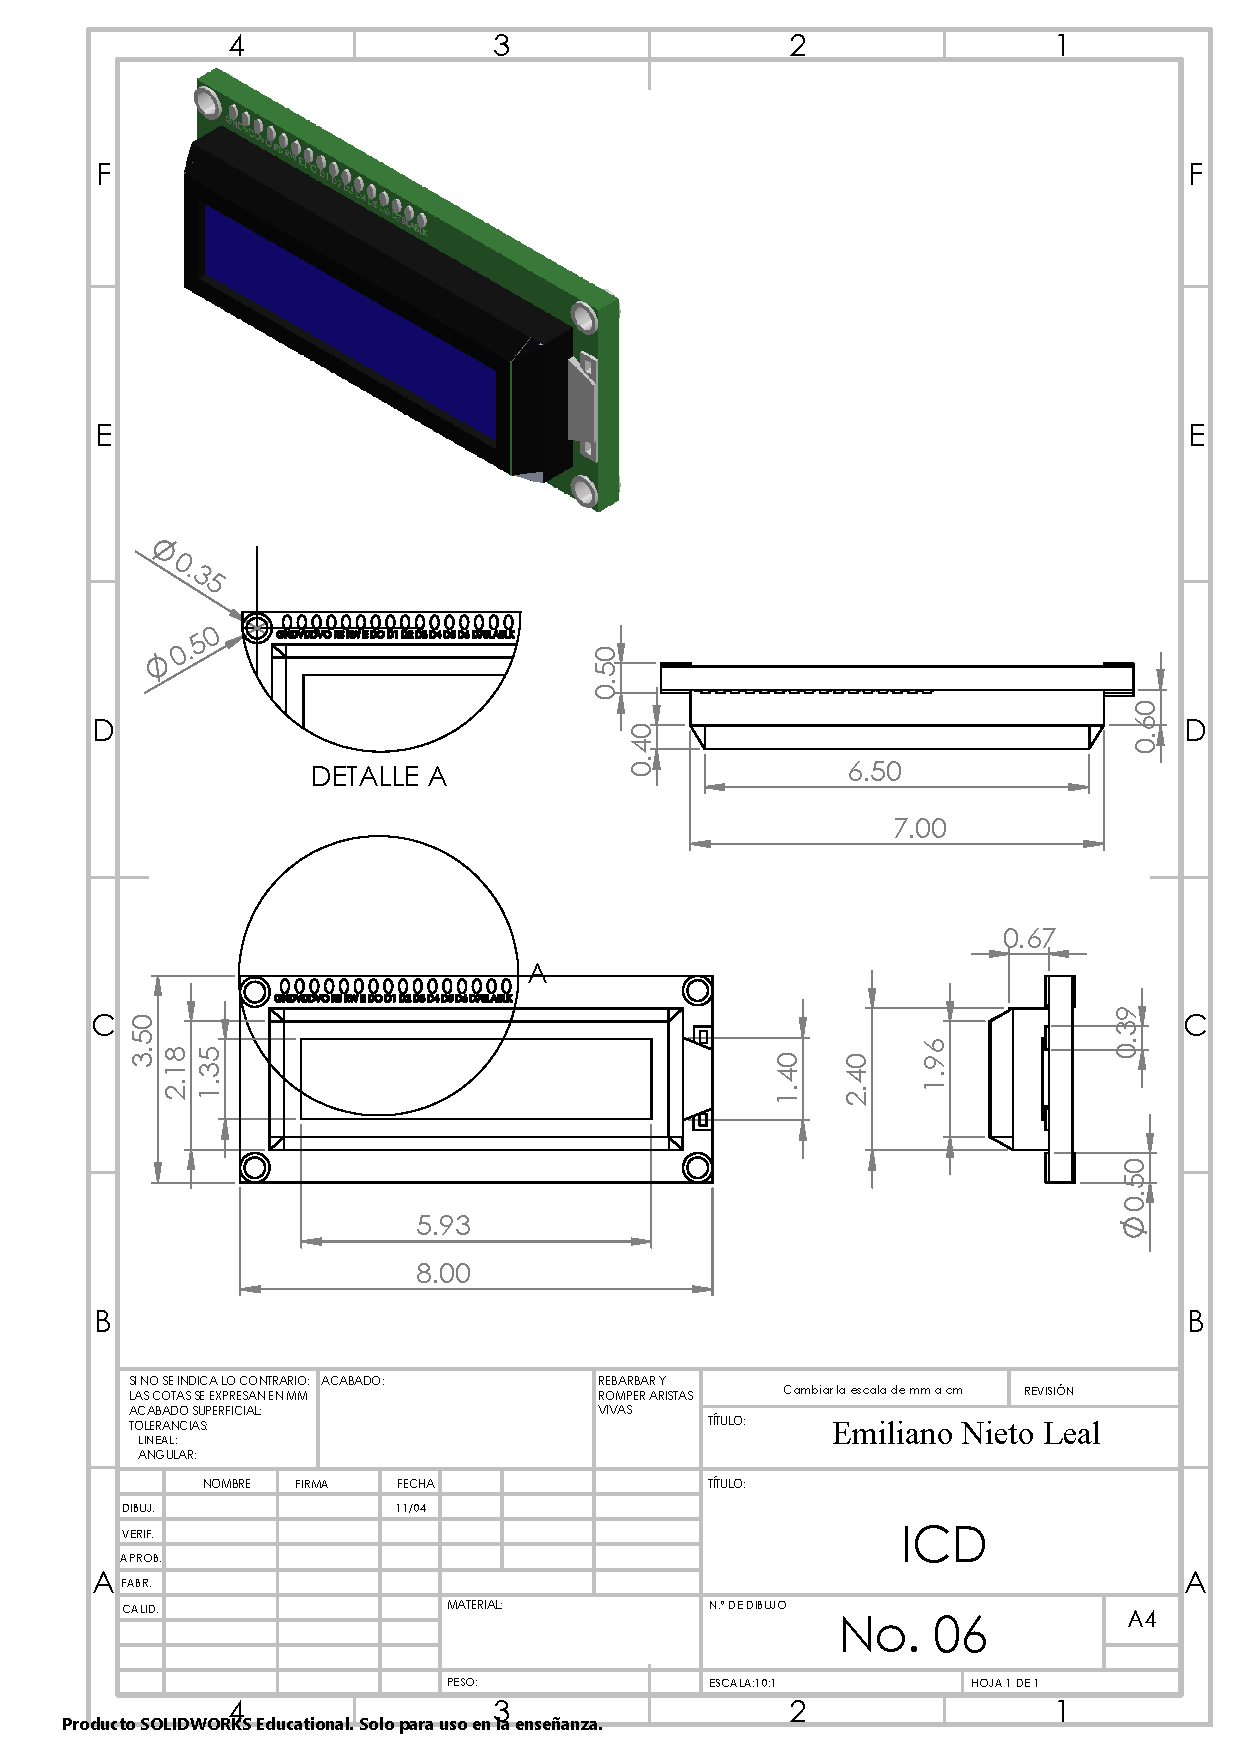
\includegraphics[trim = {1mm 1mm 1mm 1mm},clip,scale=0.5]{19/Img/icdDibujo.pdf}
        \caption{Dibujo LCD}
        \label{fig:Dibujo LCD}
    \end{figure}
                \newpage
                \begin{figure}[H]
        \centering
        \includegraphics[trim = {1mm 1mm 1mm 1mm},clip,scale=0.5]{19/Img/extensiónDibujo.pdf}
        \caption{Dibujo Extensión}
        \label{fig:Dibujo Extensión}
    \end{figure}
            \newpage
                \begin{figure}[H]
        \centering
        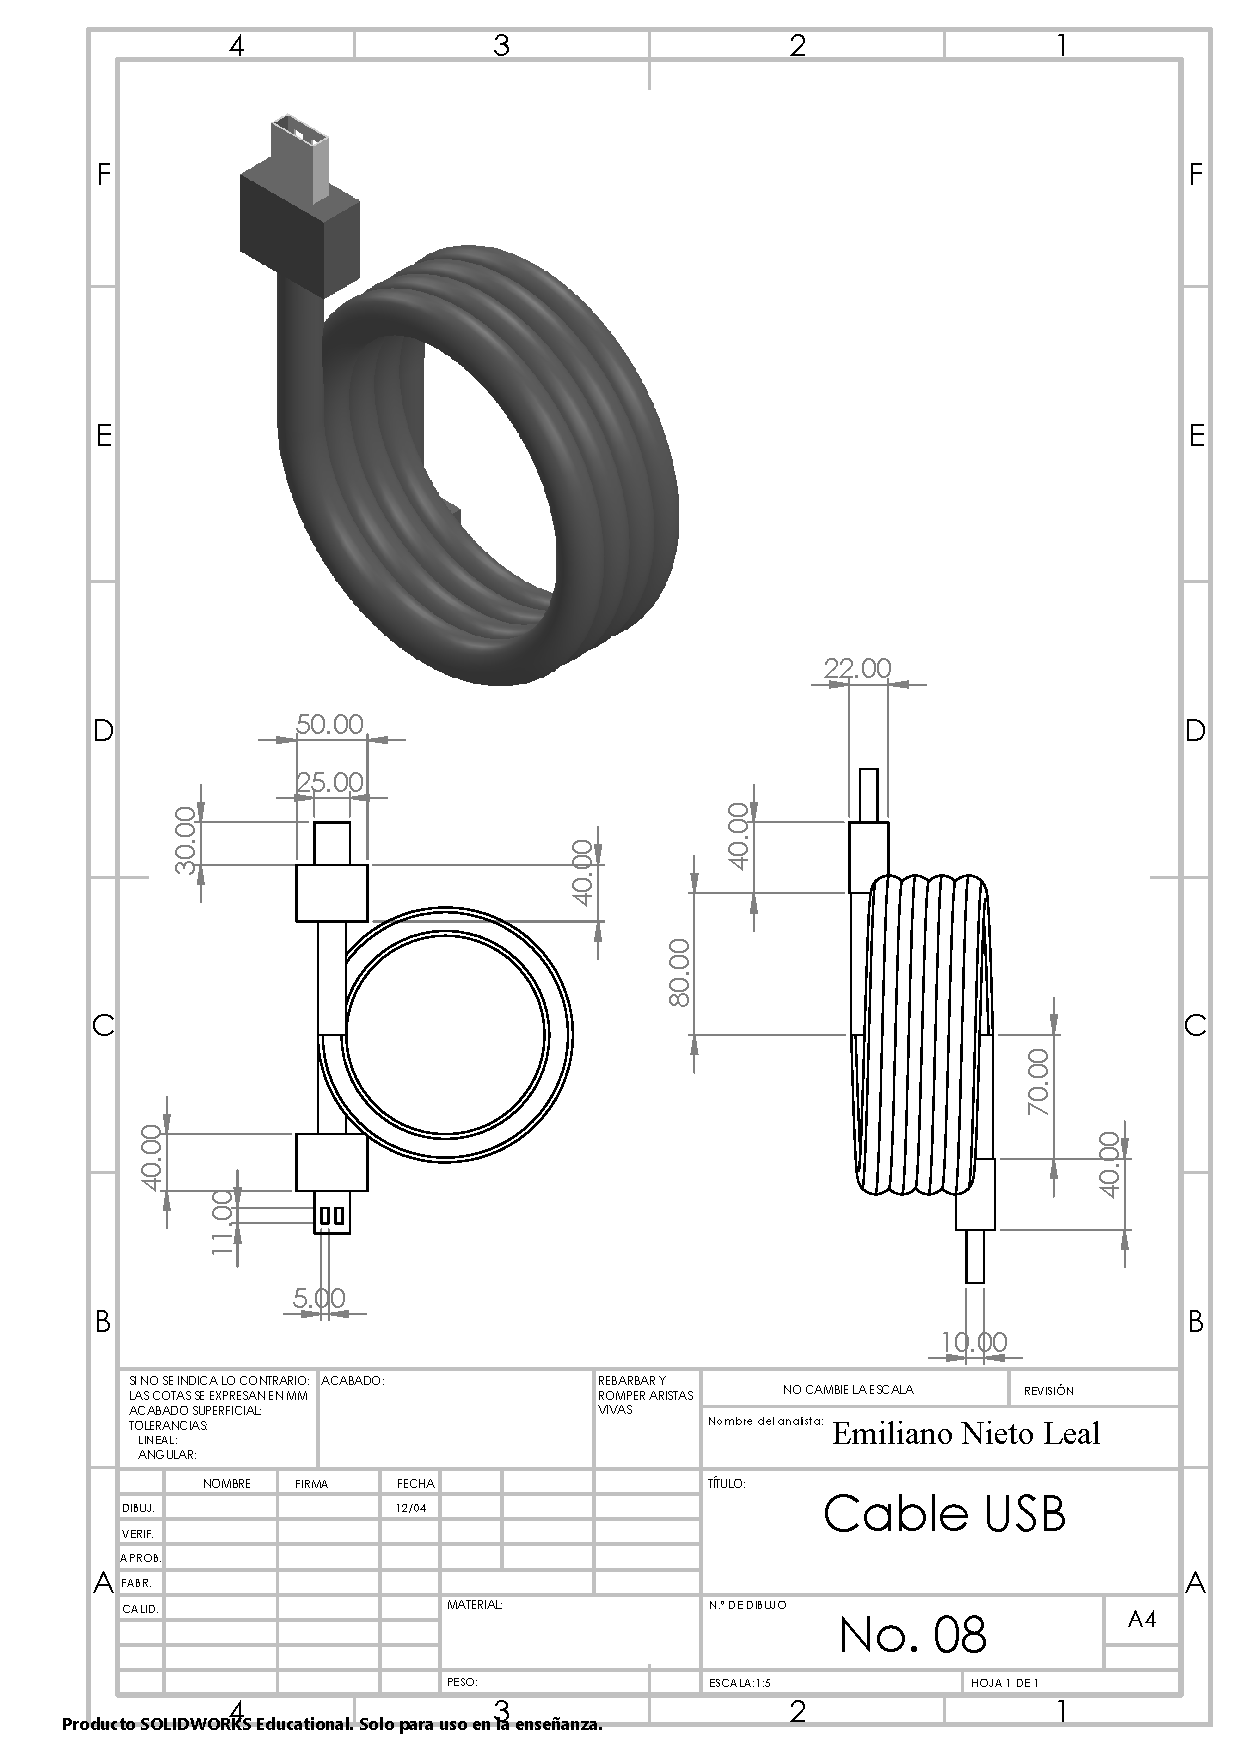
\includegraphics[trim = {1mm 1mm 1mm 1mm},clip,scale=0.5]{19/Img/cableUSBDibujo.pdf}
        \caption{Dibujo Cable USB}
        \label{fig:Dibujo CableUSB}
    \end{figure}
           \newpage
                \begin{figure}[H]
        \centering
        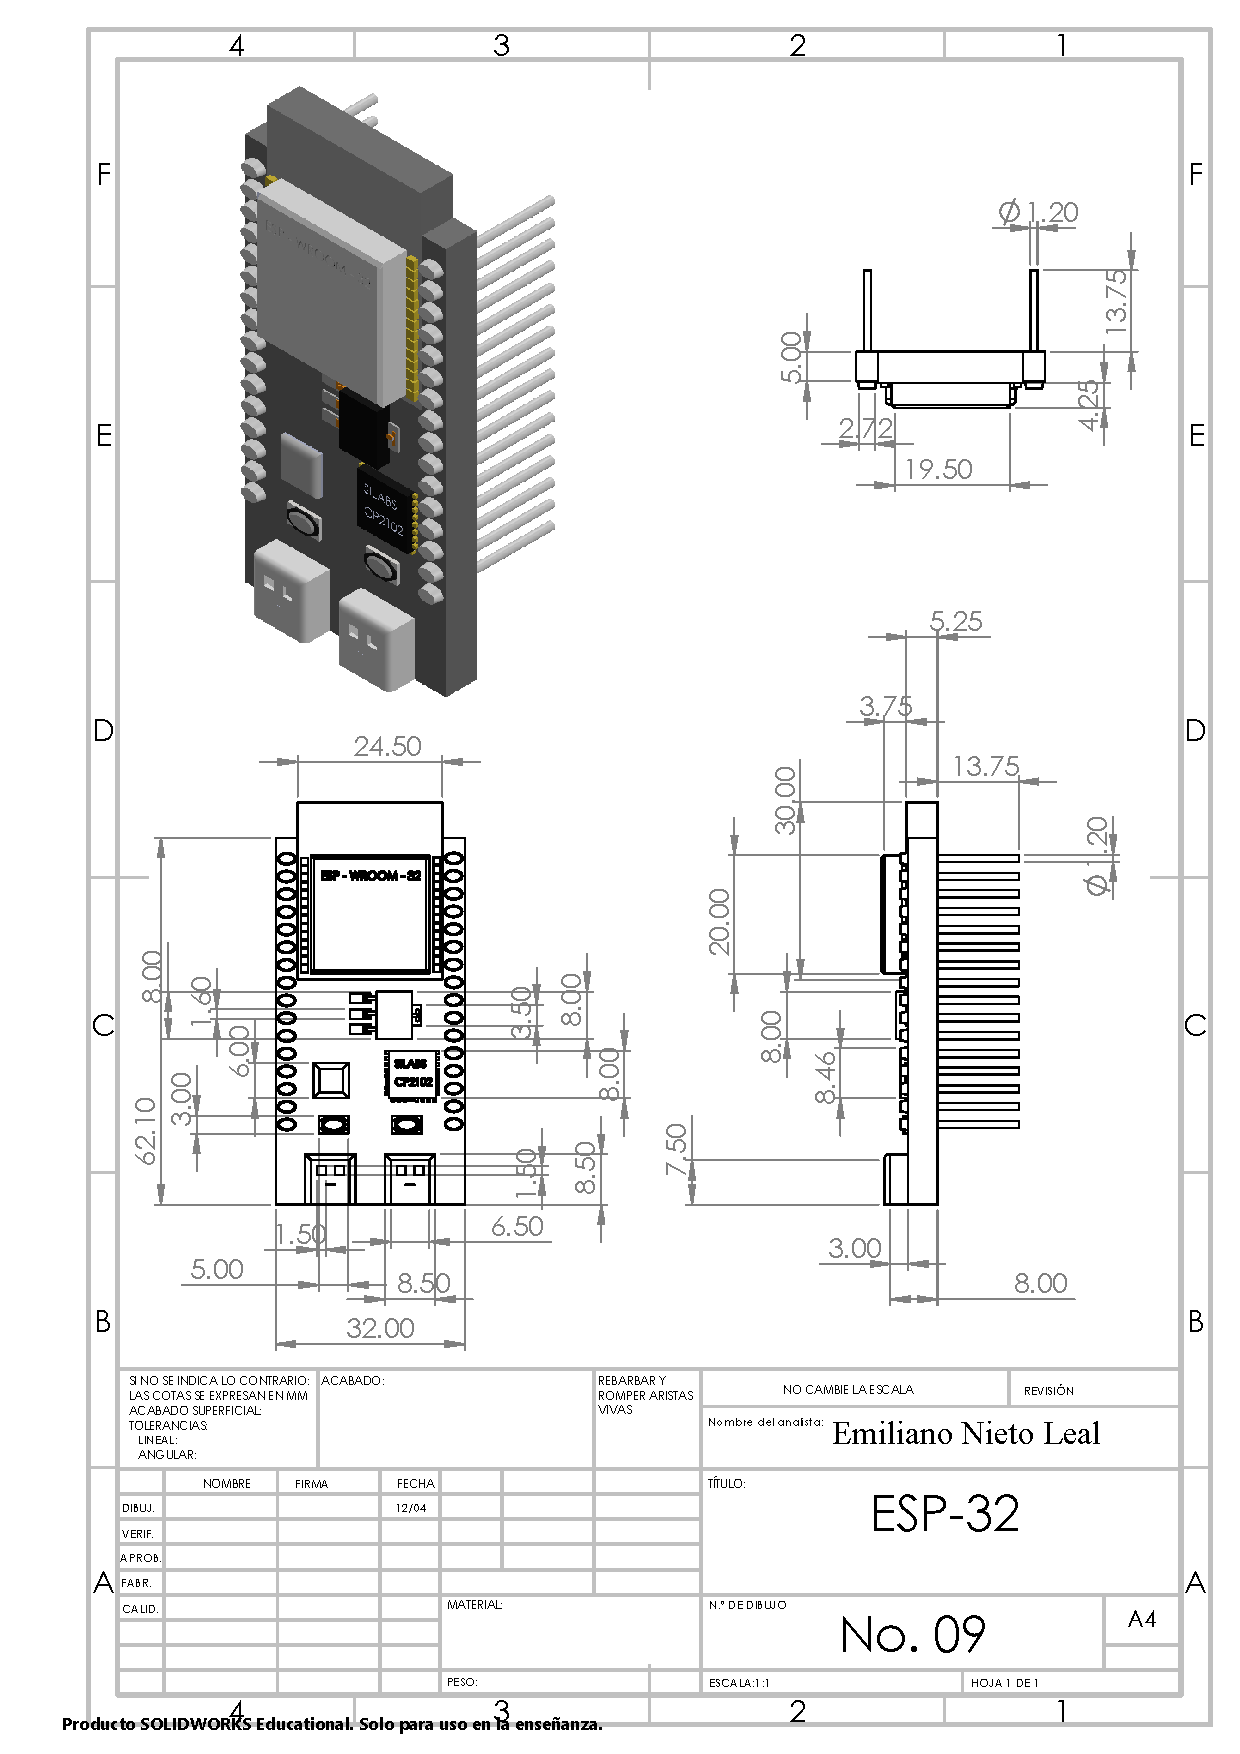
\includegraphics[trim = {1mm 1mm 1mm 1mm},clip,scale=0.5]{19/Img/esp-32Dibujo.pdf}
        \caption{Dibujo ESP-32}
        \label{fig:Dibujo ESP-32}
    \end{figure}
    
    \newpage
                \begin{figure}[H]
        \centering
        \includegraphics[trim = {1mm 1mm 1mm 1mm},clip,scale=0.5]{19/Img/móduloI2CInterfazDibujo.pdf}
        \caption{Dibujo Módulo I2C Interfaz}
        \label{fig:modulodibujo}
    \end{figure}
           
    \clearpage
    \newpage
         Estas piezas serán consideradas en la fabricación del manual para el operador, permitiendo conocer la forma de estas y el uso que se tendrá de las mismas.
         Cada pieza deberá encontrarse en un área accesible para el operador por lo que será necesario el uso de una herramienta para mantener los elementos con un orden y posición especifica, para la facilitación del operador, usando como ejemplo un tapete organizador, en donde se podrán colocar todo lo necesario para realizar el ensamble.\ref{fig:tapete}.
    
        \begin{figure}[H]
        \centering
        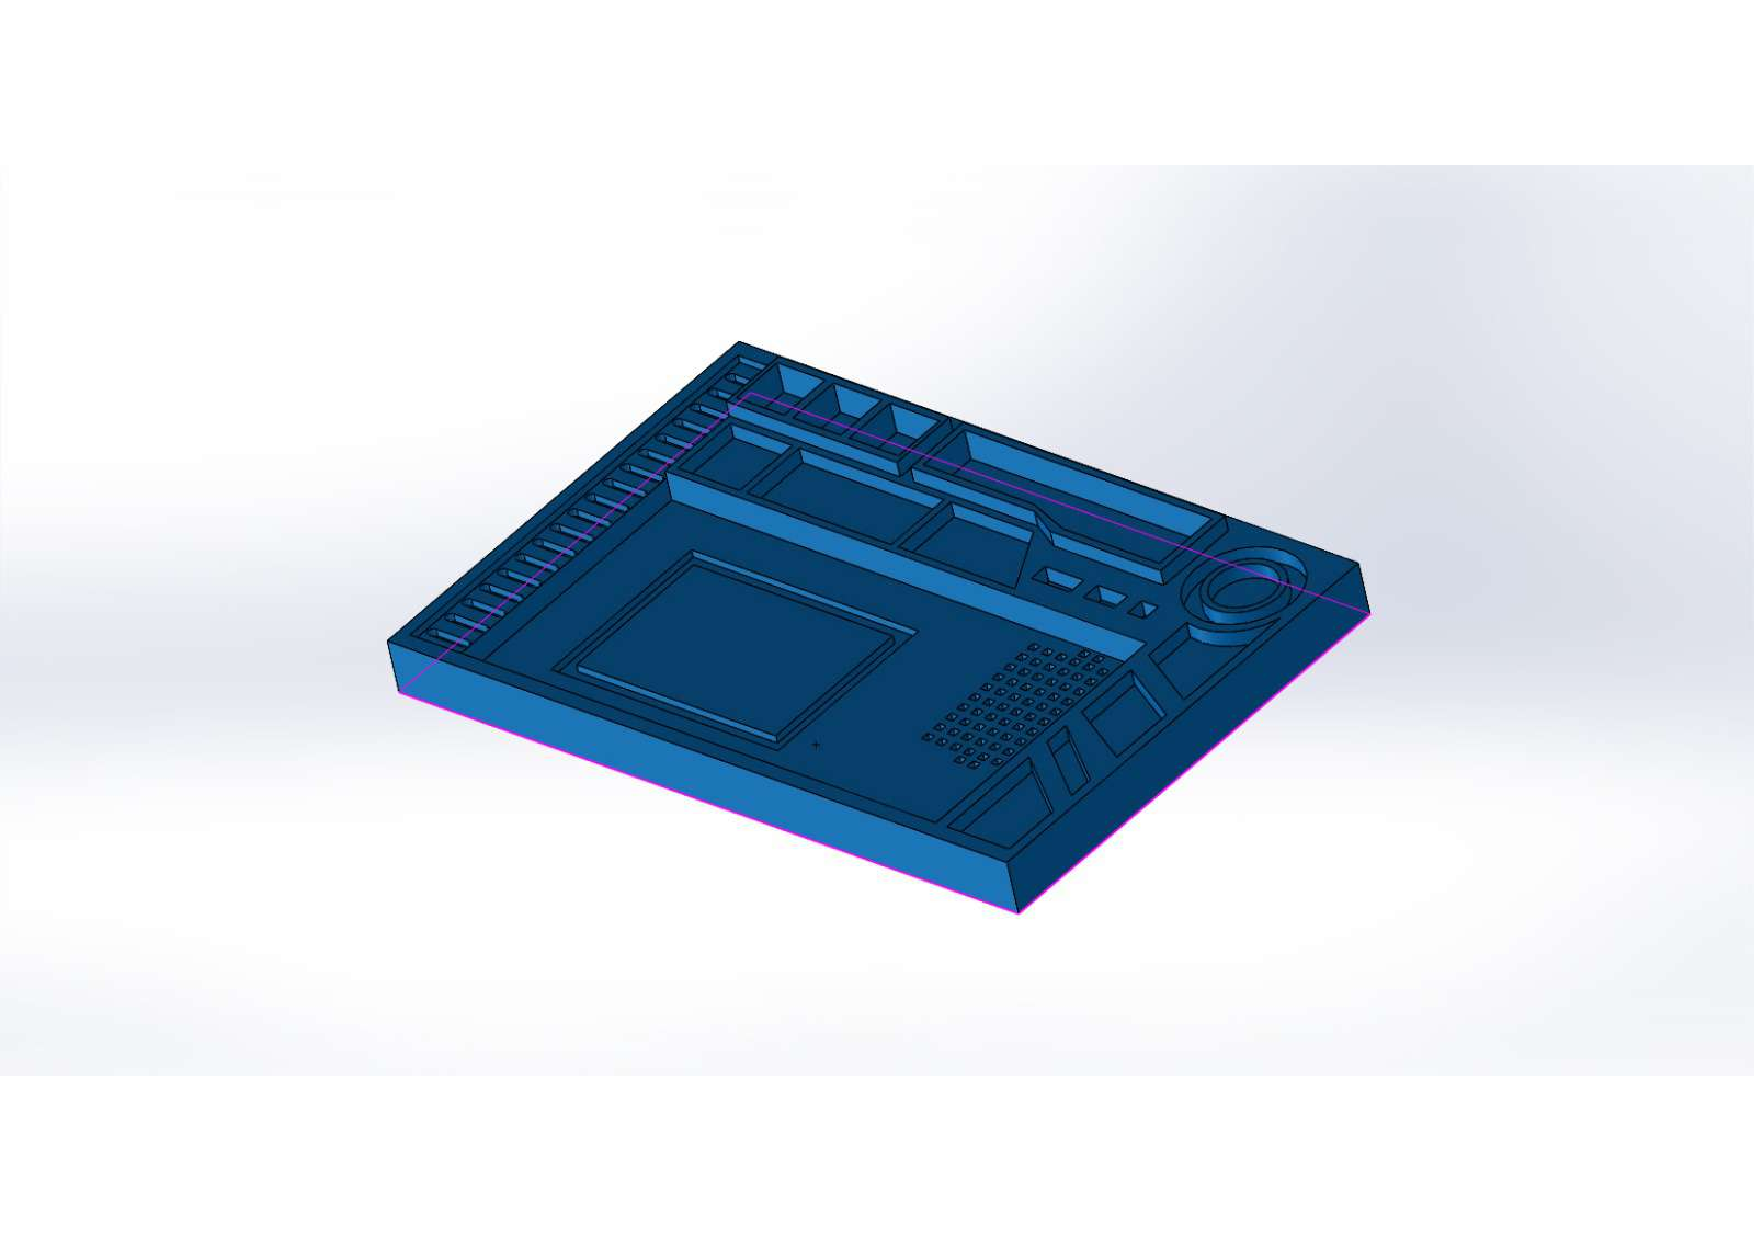
\includegraphics[trim = {65mm 55mm 65mm 55mm},clip,scale=0.5]{19/Img/tapeteOrganizadorFigura.pdf}
        \caption{Imagen del modelo 3D del Tapete organizador}
        \label{fig:tapete}
    \end{figure}
    
    \newpage
                \begin{figure}[H]
        \centering
        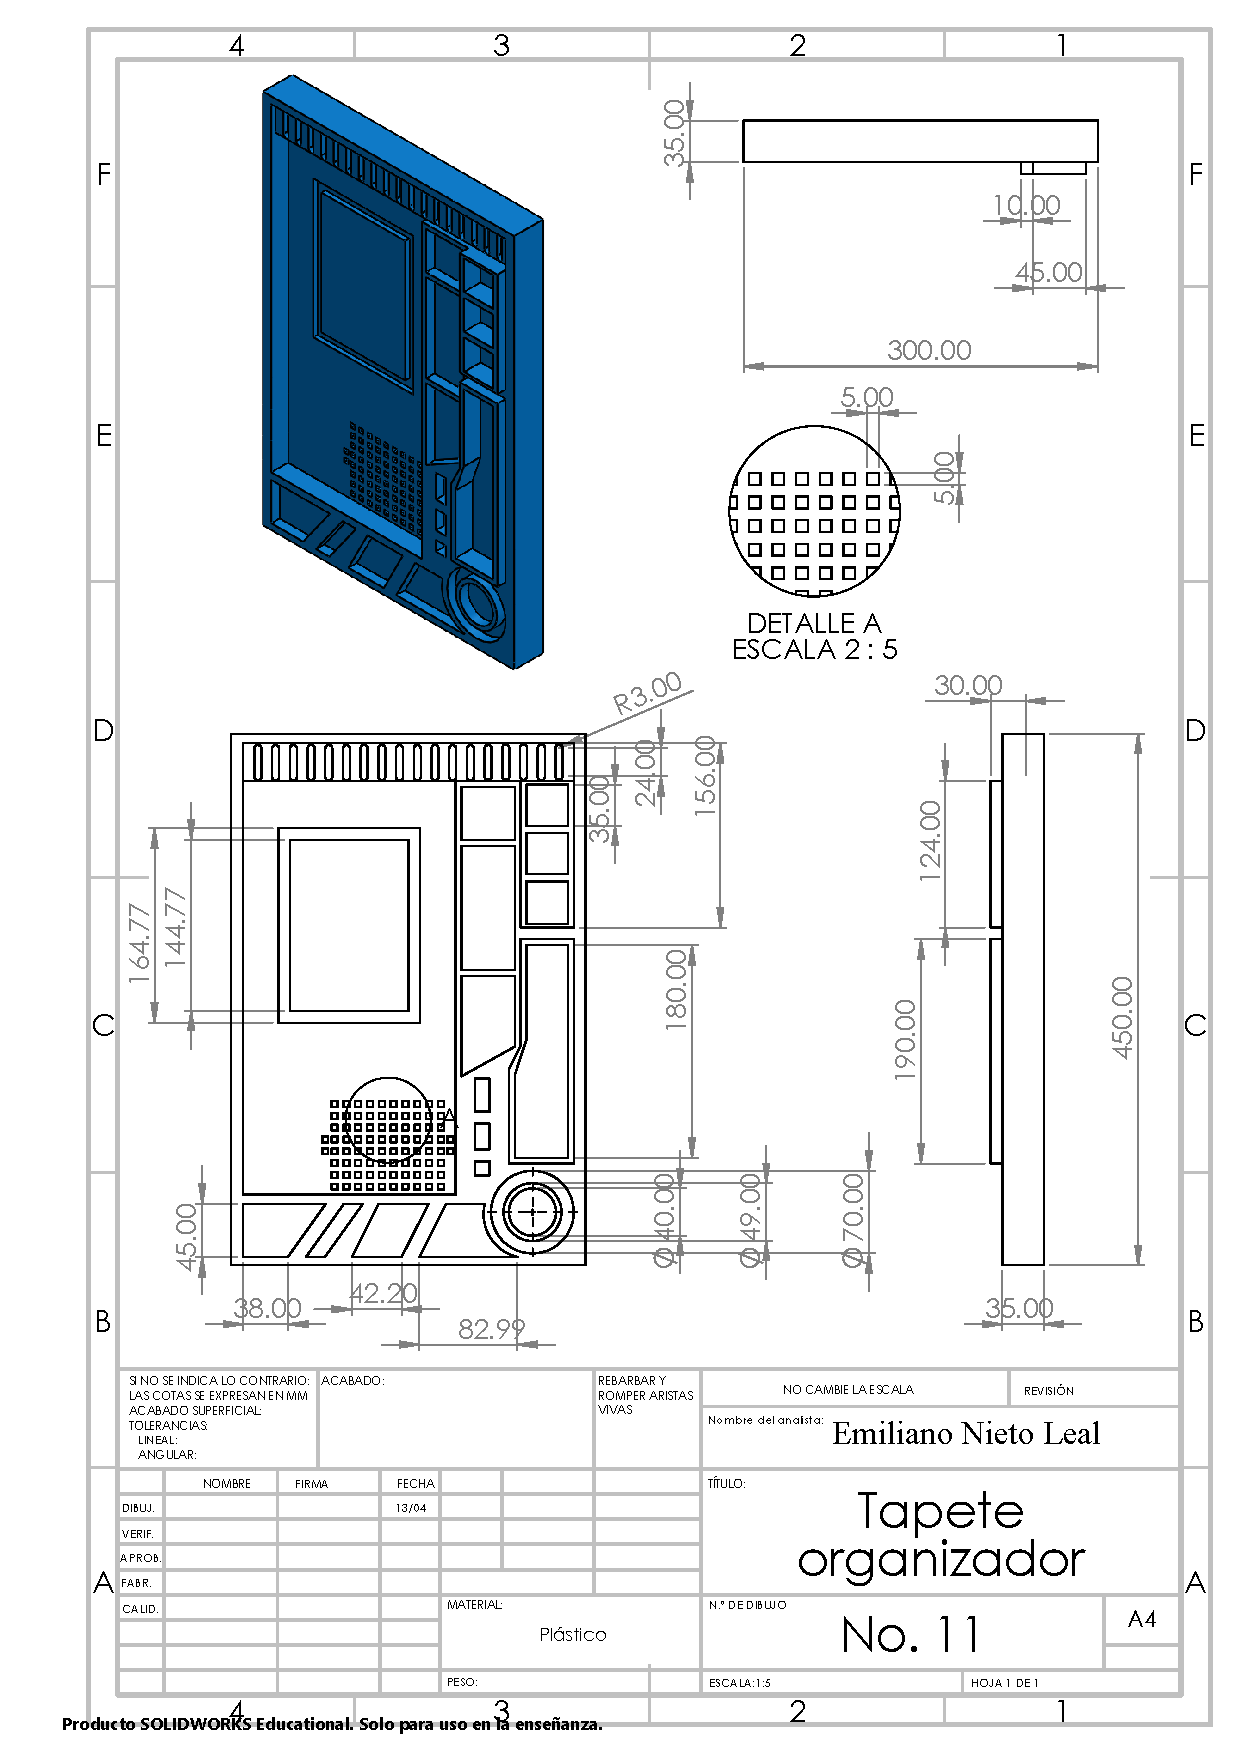
\includegraphics[trim = {1mm 1mm 1mm 1mm},clip,scale=0.5]{19/Img/tapeteOrganizadorDibujo.pdf}
        \caption{Dibujo Tapete Organizador}
        \label{fig:tapeteOrganizador}
    \end{figure}
    
    
        Después del operario entender los pasos y el proceso que se llevará acaba para realizar el ensamble se pedirá al operario que recuerde la cantidad de piezas a ocupar de cada material y cual es la función d esta en el circuito a ensamblar.
        \\Posterior a ello se pedirá que coloque todas las piezas y materiales necesarios para el proceso del ensamblaje en una posición adecuada alrededor del Tapete organizador como se presenta a continuación.\ref{fig:ensamblaje1}.
    \begin{figure}[H]
        \centering
        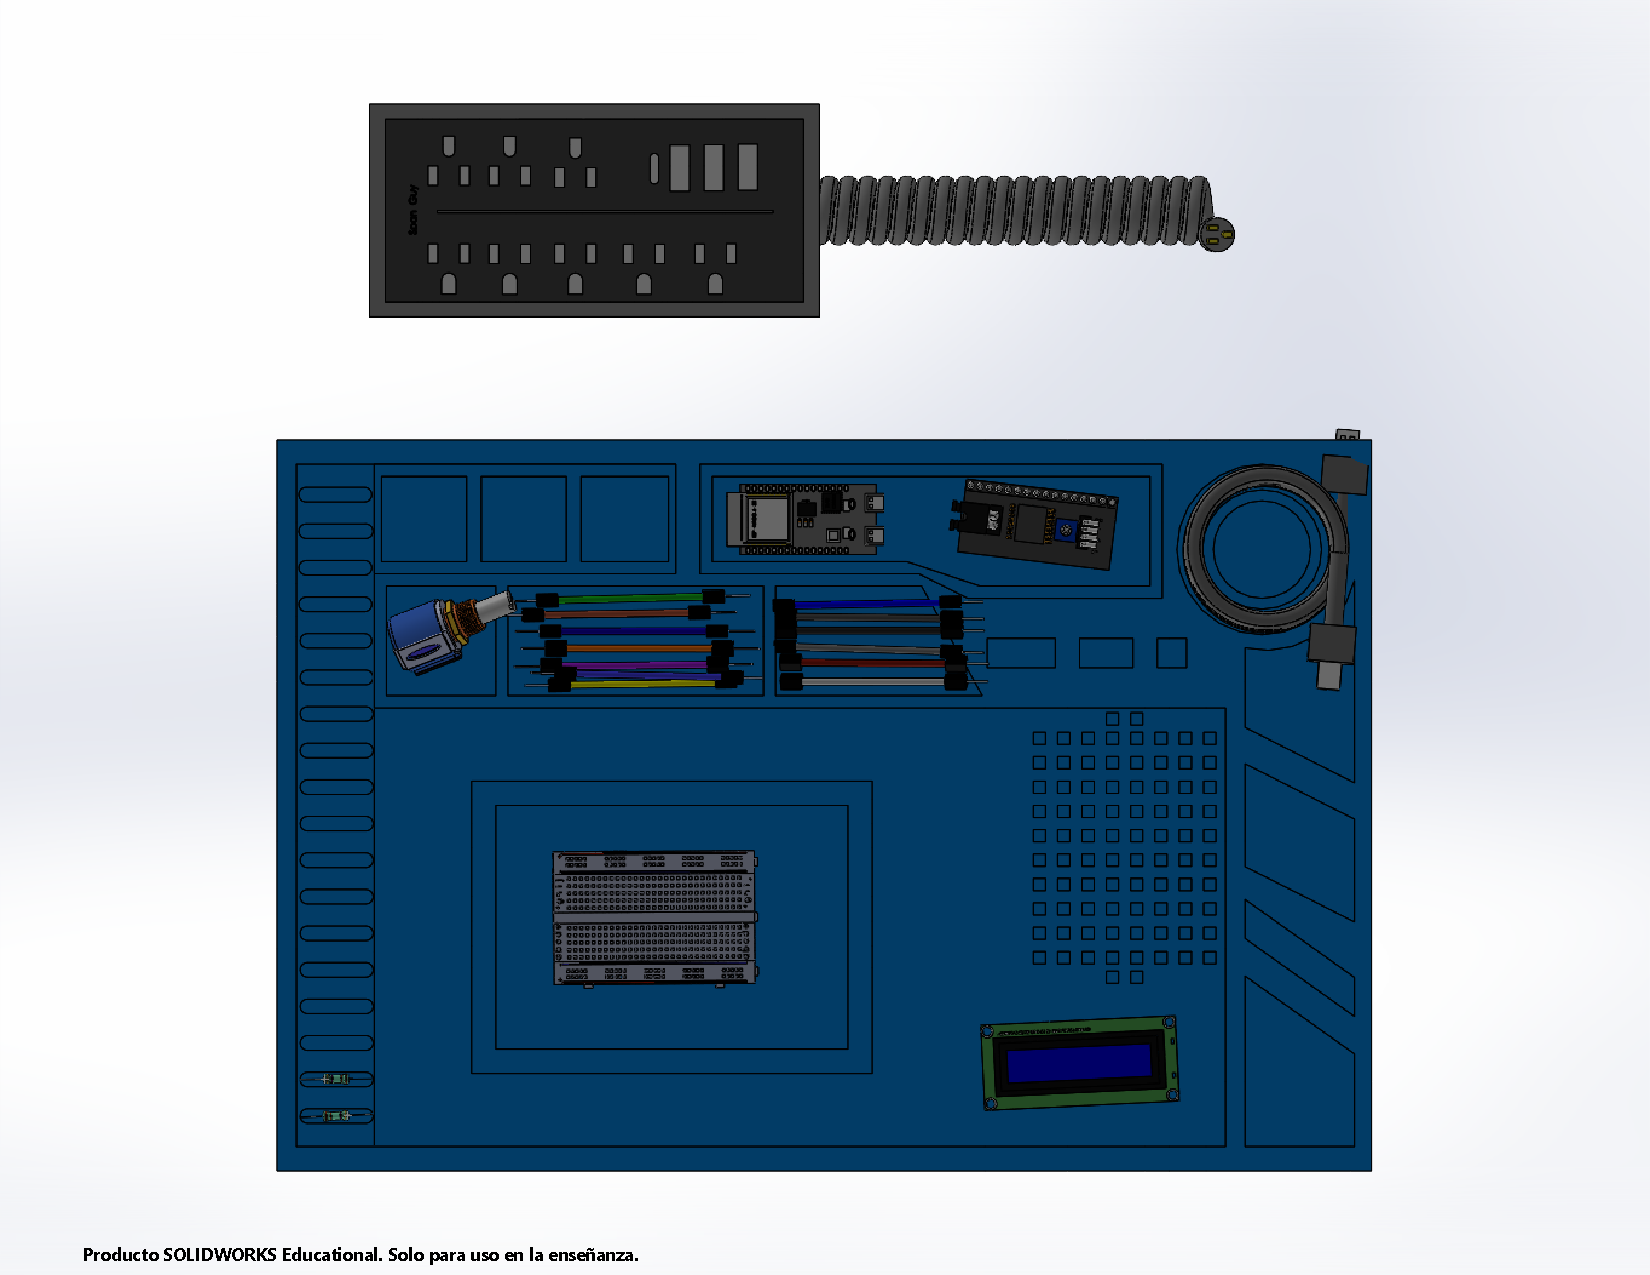
\includegraphics[trim = {55mm 15mm 48mm 20mm},clip,scale=0.5]{19/Img/ensamblaje1.pdf}
        \caption{Dibujo del Tapete Organizador con todas las piezas en orden}
        \label{fig:ensamblaje1}
    \end{figure}

        
         Después el operador dará inicio al proceso, con el inicio del operario el analista esta preparado con una cámara de vídeo con la cual se grabará la película en la cual podamos ver el proceso a realizar y la confirmación de haber realizado la prueba de calidad del producto.
        Al concluir este proceso con la confirmación de la prueba se terminará la primera observación, posteriormente el mismo analista deberá de llevar acabo una segunda observación para luego tomar el rol de operador, el cual igualmente ensamblara dos veces el circuito para obtener los valores  de cada observación usando la  fórmula para el valor esperado, el cual consiste en:
    
        \begin{equation}
        \label{eq1}
        (x1+x2+x3+........+xn)/n 
    \end{equation}
    
        para así poder obtener la media de todos los tiempos y concluir que este este es el tiempo esperado que se obtendrá al llevar acabo la metodología de tiempos continuos y de esta manera compararla con la siguiente metodología.
     
    
    %\subsection{Prepara tu documento}
    
    %Antes de que comiences a utilizar esta plantilla, es recomendable que prepare la información que contendrá en un archivo aparte. 
    %Ten preparadas tus gráficas, así como también las tablas aparte, para que sea más fácil integrarlo. 
    %Se recomienda fuertemente el uso de \textbf{formato Enhanced Metafile (.emf) para imágenes y gráficas} de resolución óptima. 
    %Finalmente, completa y organiza el contenido antes de darle el formato de esta plantilla. 
    
    %\subsection{Acrónimos y Abreviaciones}

    
    %Los acrónimos y abreviaciones deberán ser definidos únicamente la primera vez que aparecen en el texto, esto para que el lector entienda lo que significan.
    
    
    \section{Resultados y discusión}
    
    Posterior a la  lectura, análisis y memorización del manual de fabricación por parte del operador se iniciara de manera manual el ensamblaje del circuito a manos del operador, buscando que el analista observe y realice la película (muestra continua) sobre como el operario llevo acabo todo el proceso de ensamblaje utilizando únicamente como base las instrucciones dadas con anterioridad, sin ningún tipo de apoyo externo, para de esta manera concluir si el circuito fue armado correctamente.
    \\Al terminar todo el proceso de armado para confirmar que este se realizo adecuadamente se necesitará que el operador realice una modificación al rango del potenciómetro, al moverlo y modificar su resistencia para observar su cambio en la pantalla, de esta manera el analista deberá de tomar evidencia de como no solo la pantalla LCD funciona adecuadamente al prender y enviar una señal, sino también el hecho de que si se genera algún cambio en la lectura ofrecida por el potenciómetro a la hora de variar la resistencia de este último como se observa en la siguiente imagen\ref{fig:evidenciaCambio1}.
                \begin{figure}[H]
        \centering
        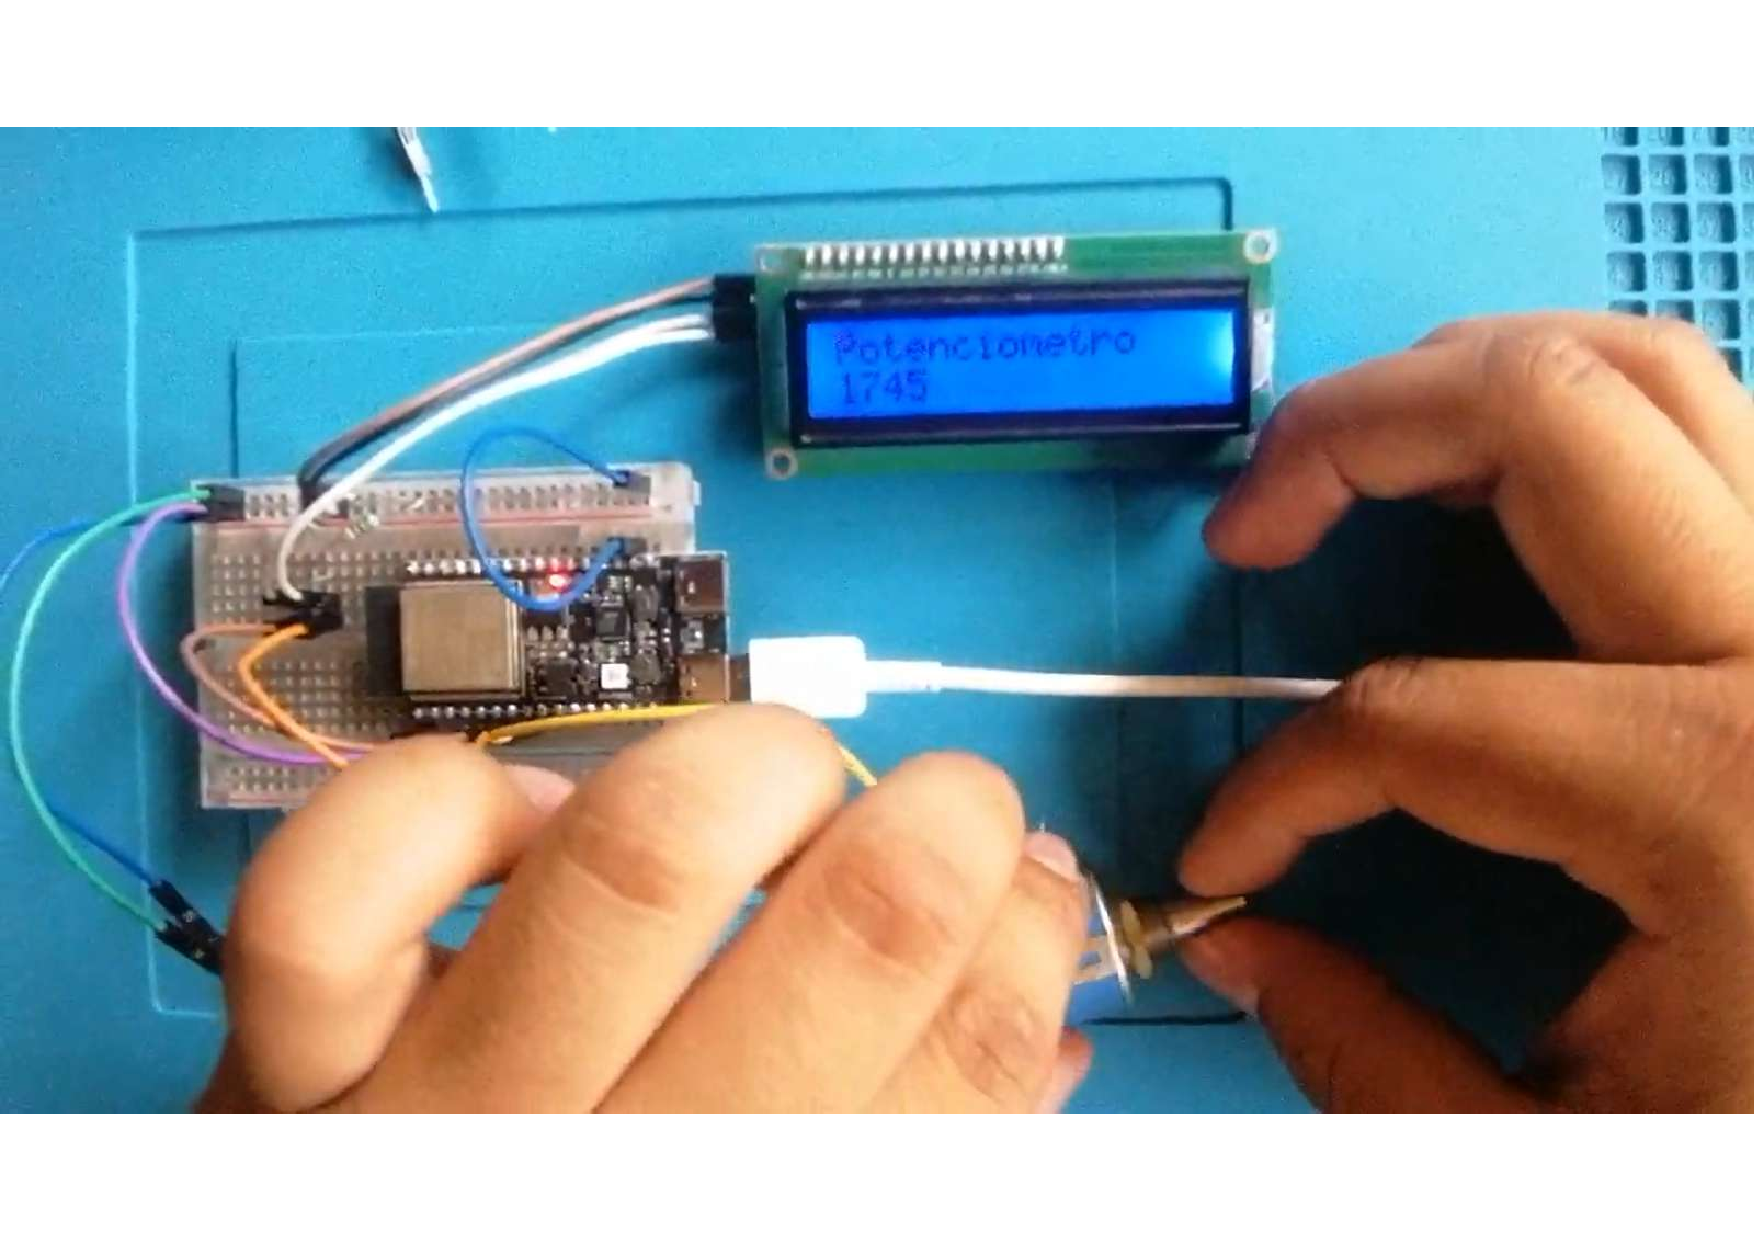
\includegraphics[trim = {45mm 15mm 80mm 20mm},clip,scale=0.5]{19/Img/evidenciaCambio1.pdf}
        \caption{Primer lectura obtenida a la hora de armar el circuito.}
        \label{fig:evidenciaCambio1}
    \end{figure}
    Como se puede observar en la figura \ref{fig:evidenciaCambio1} se puede confirmar como al realizar el ensamble usando como base el manual realizado se logro no solo que se generará una señal a la pantalla, sino además como se muestra en la figura \ref{fig:evidenciaCambio2} se puede confirmar que a la hora de mover el potenciómetro este efectivamente cambio el valor presentado en el LCD.
                    \begin{figure}[H]
        \centering
        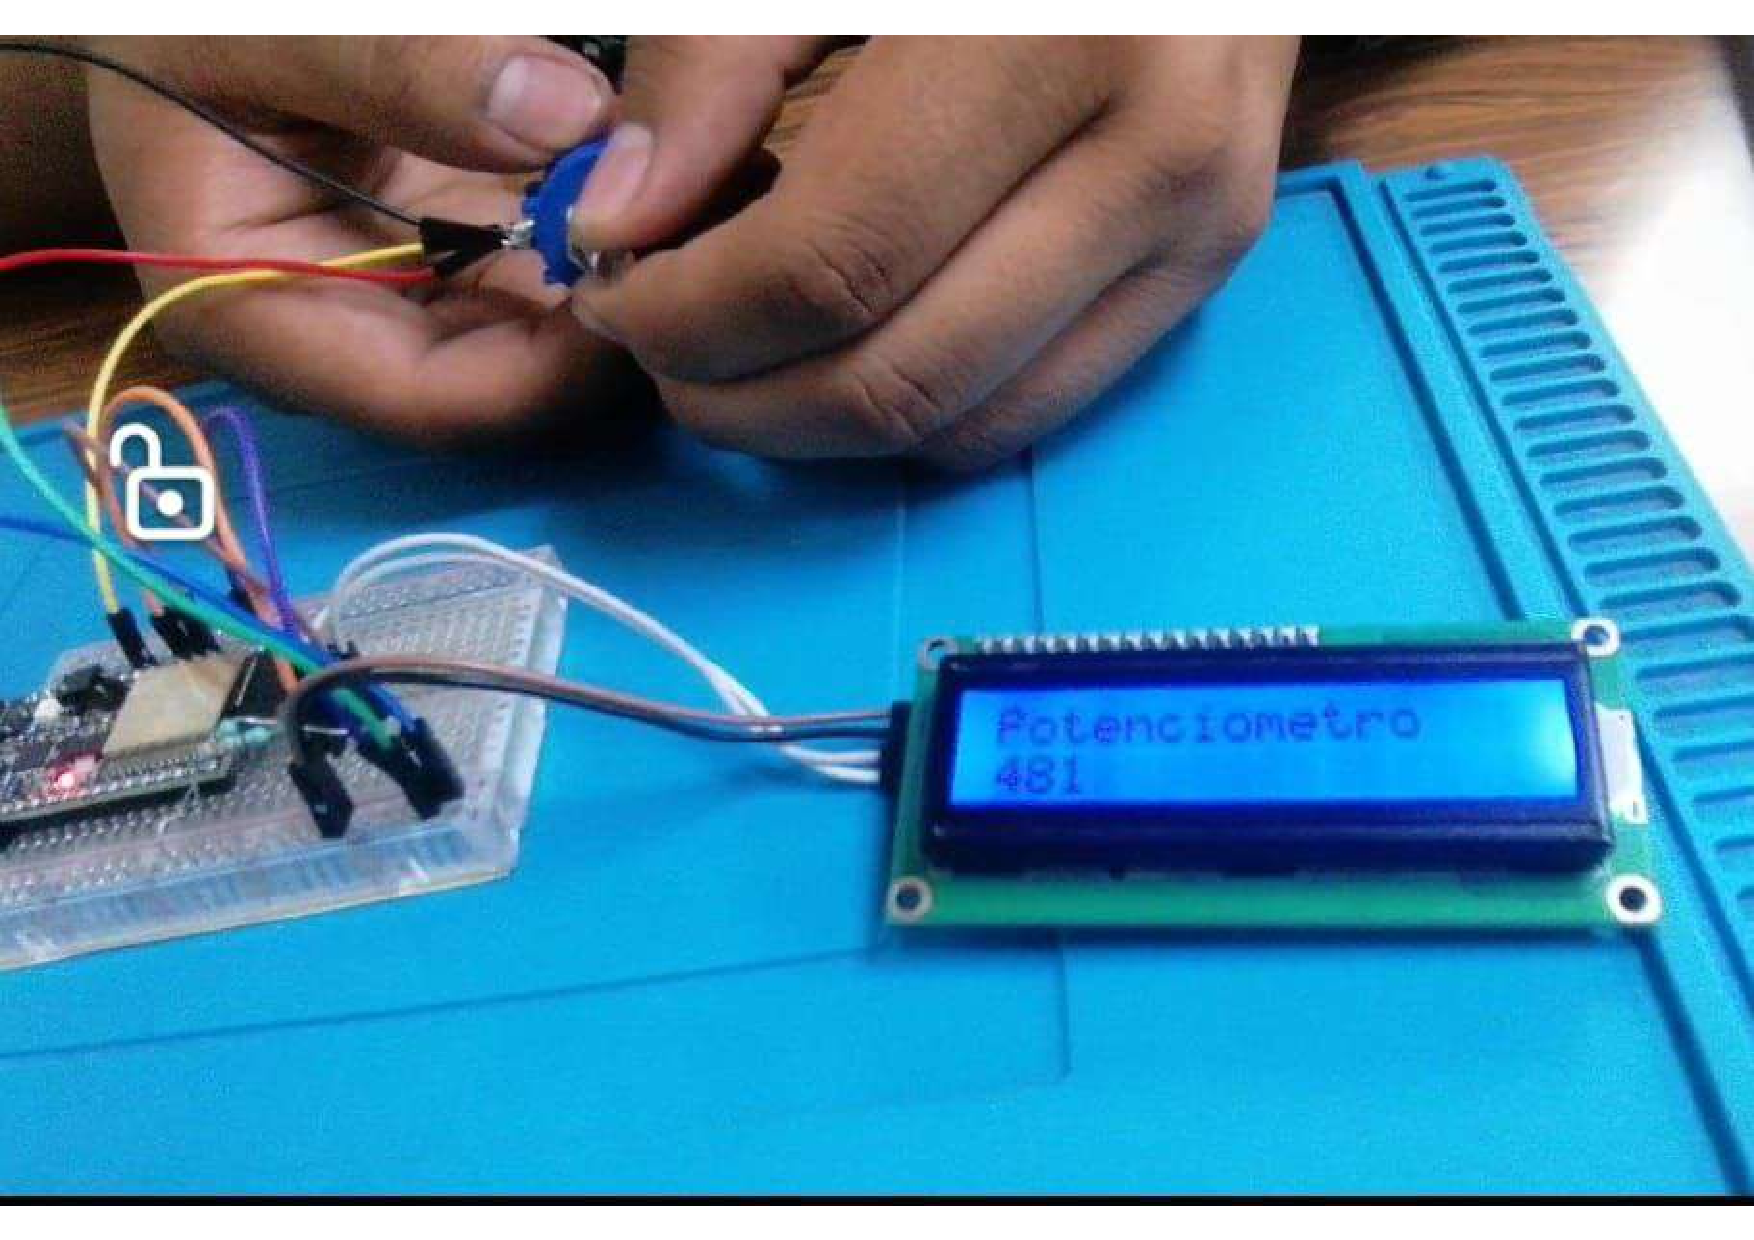
\includegraphics[trim = {45mm 15mm 80mm 20mm},clip,scale=0.5]{19/Img/evidenciaCambio2.pdf}
        \caption{Segunda lectura obtenida a la hora de armar el circuito.}
        \label{fig:evidenciaCambio2}
    \end{figure}
    Continuando con el mismo proceso se realizaron otras cuatro modificaciones al valor de la resistencia del potenciómetro para de esta manera tener evidencia sólida de que la modificación y todo el proceso fue el adecuado, demostrado en las siguientes figuras:
    \newpage
    \begin{figure}[H]
        \centering
        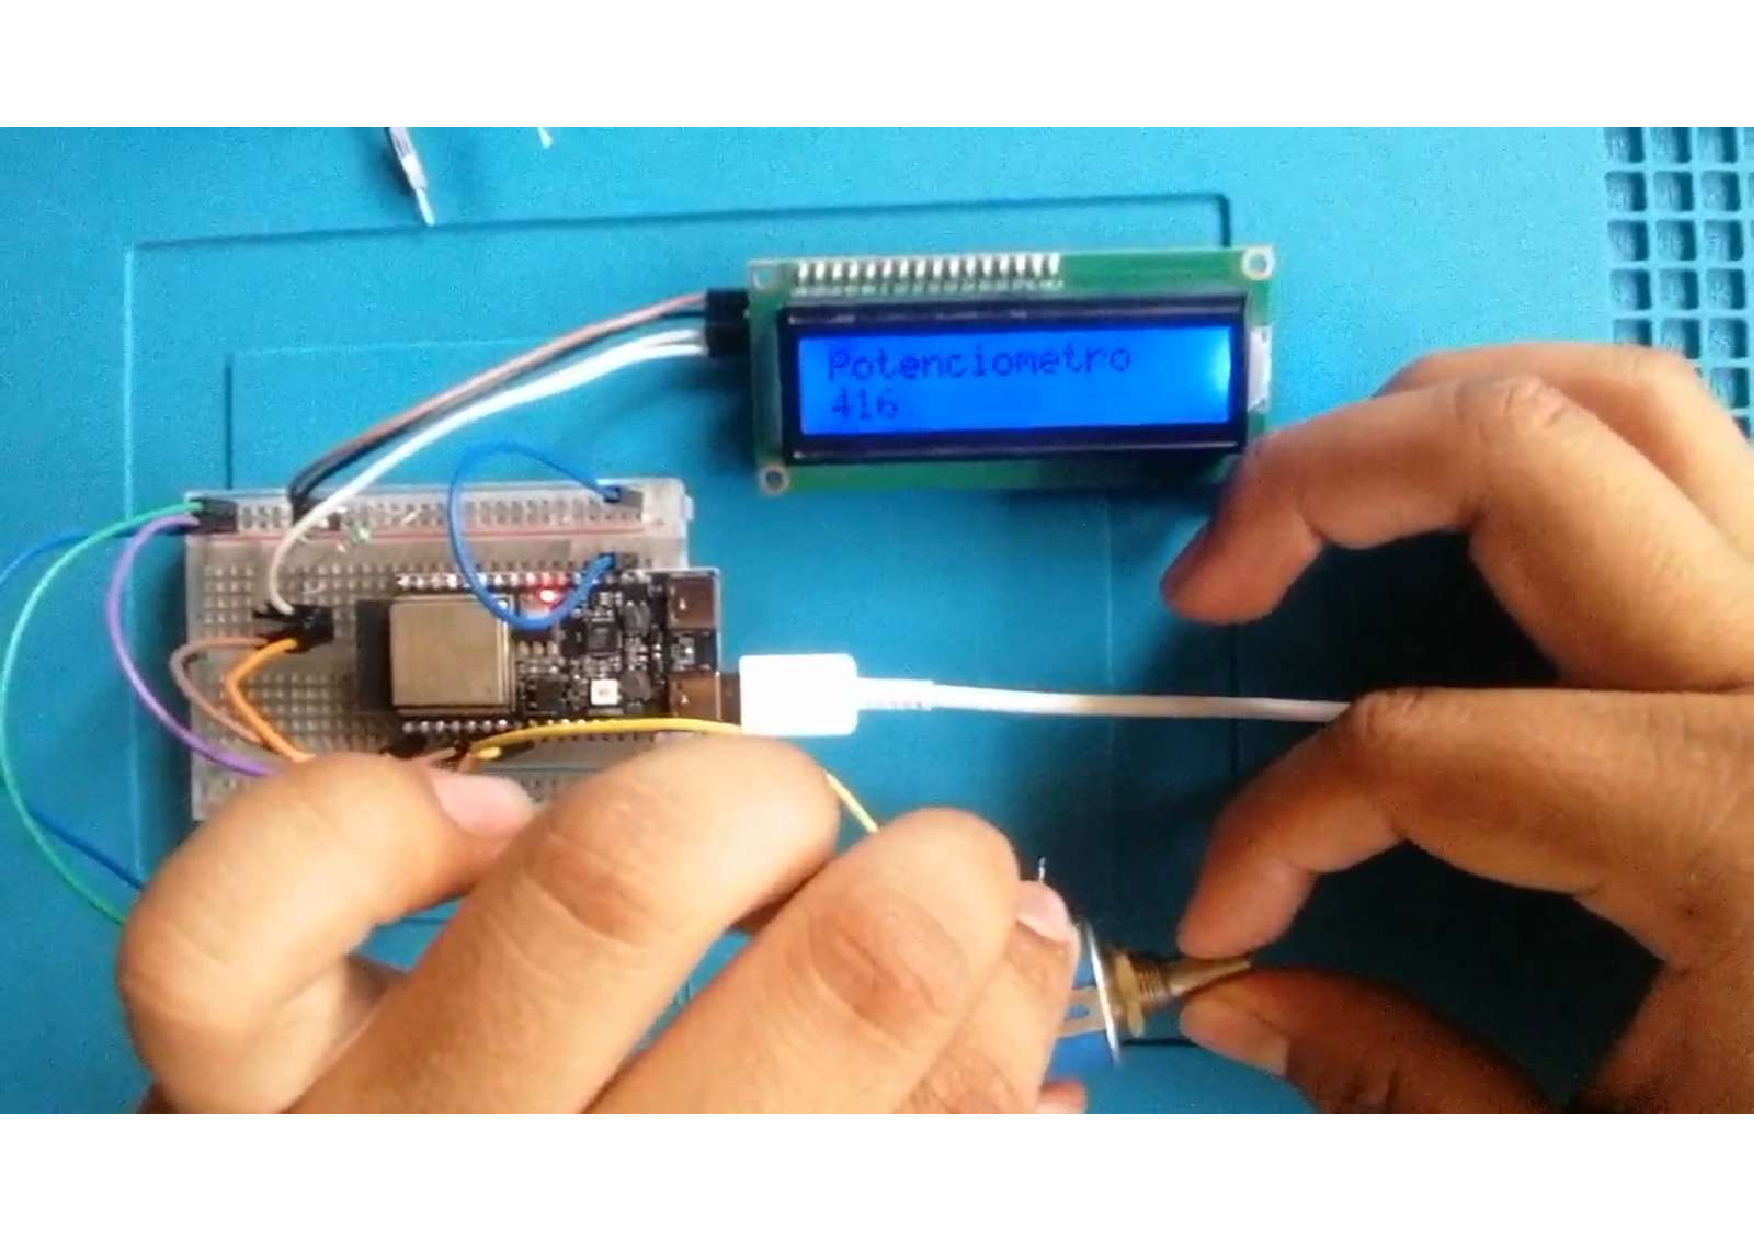
\includegraphics[trim = {45mm 15mm 80mm 20mm},clip,scale=0.5]{19/Img/evidenciaCambio3.pdf}
        \caption{Tercera lectura obtenida a la hora de armar el circuito.}
        \label{fig:evidenciaCambio3}
    \end{figure}
\begin{figure}[H]
        \centering
        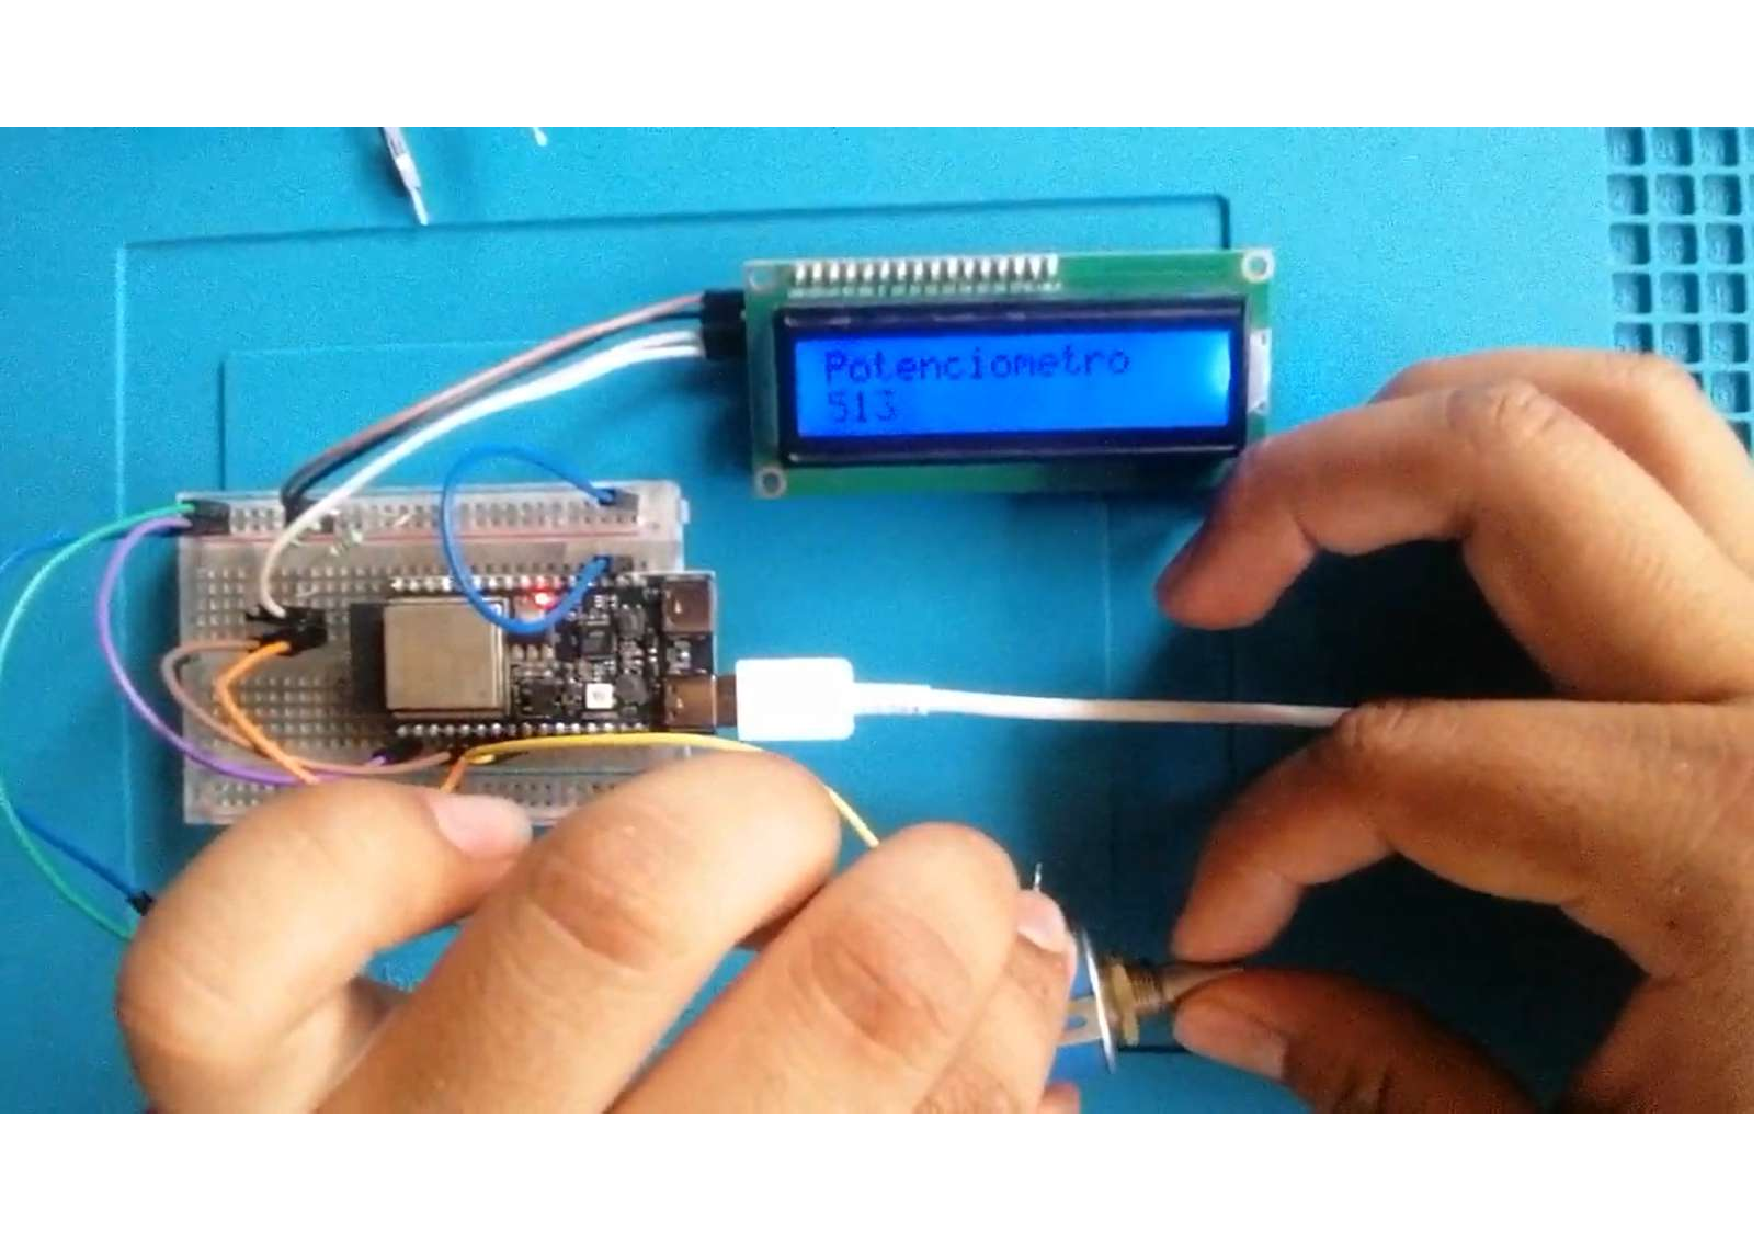
\includegraphics[trim = {45mm 15mm 80mm 20mm},clip,scale=0.5]{19/Img/evidenciaCambio4.pdf}
        \caption{Cuarta lectura obtenida a la hora de armar el circuito.}
        \label{fig:evidenciaCambio4}
    \end{figure}
        \begin{figure}[H]
        \centering
        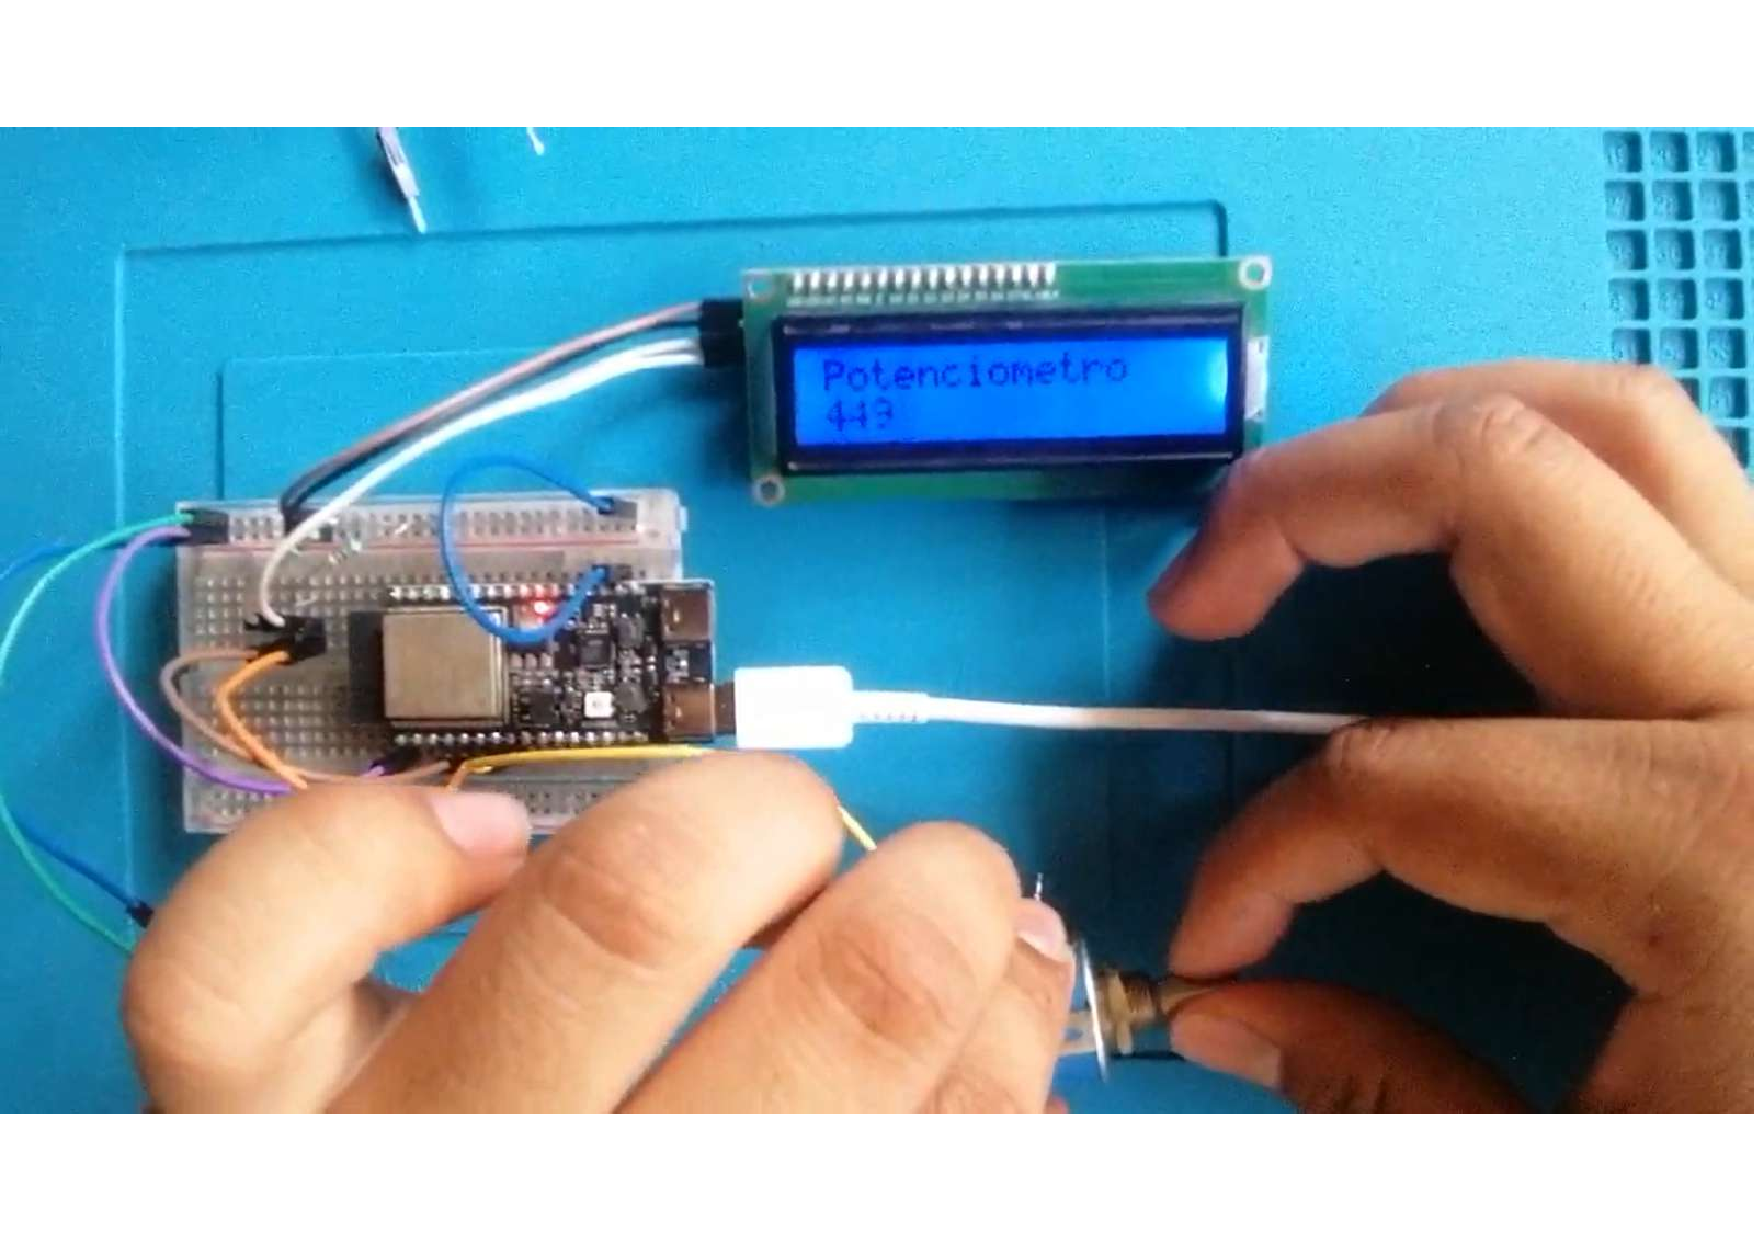
\includegraphics[trim = {45mm 15mm 80mm 20mm},clip,scale=0.5]{19/Img/evidenciaCambio5.pdf}
        \caption{Quinta lectura obtenida a la hora de armar el circuito.}
        \label{fig:evidenciaCambio5}
    \end{figure}
\begin{figure}[H]
        \centering
        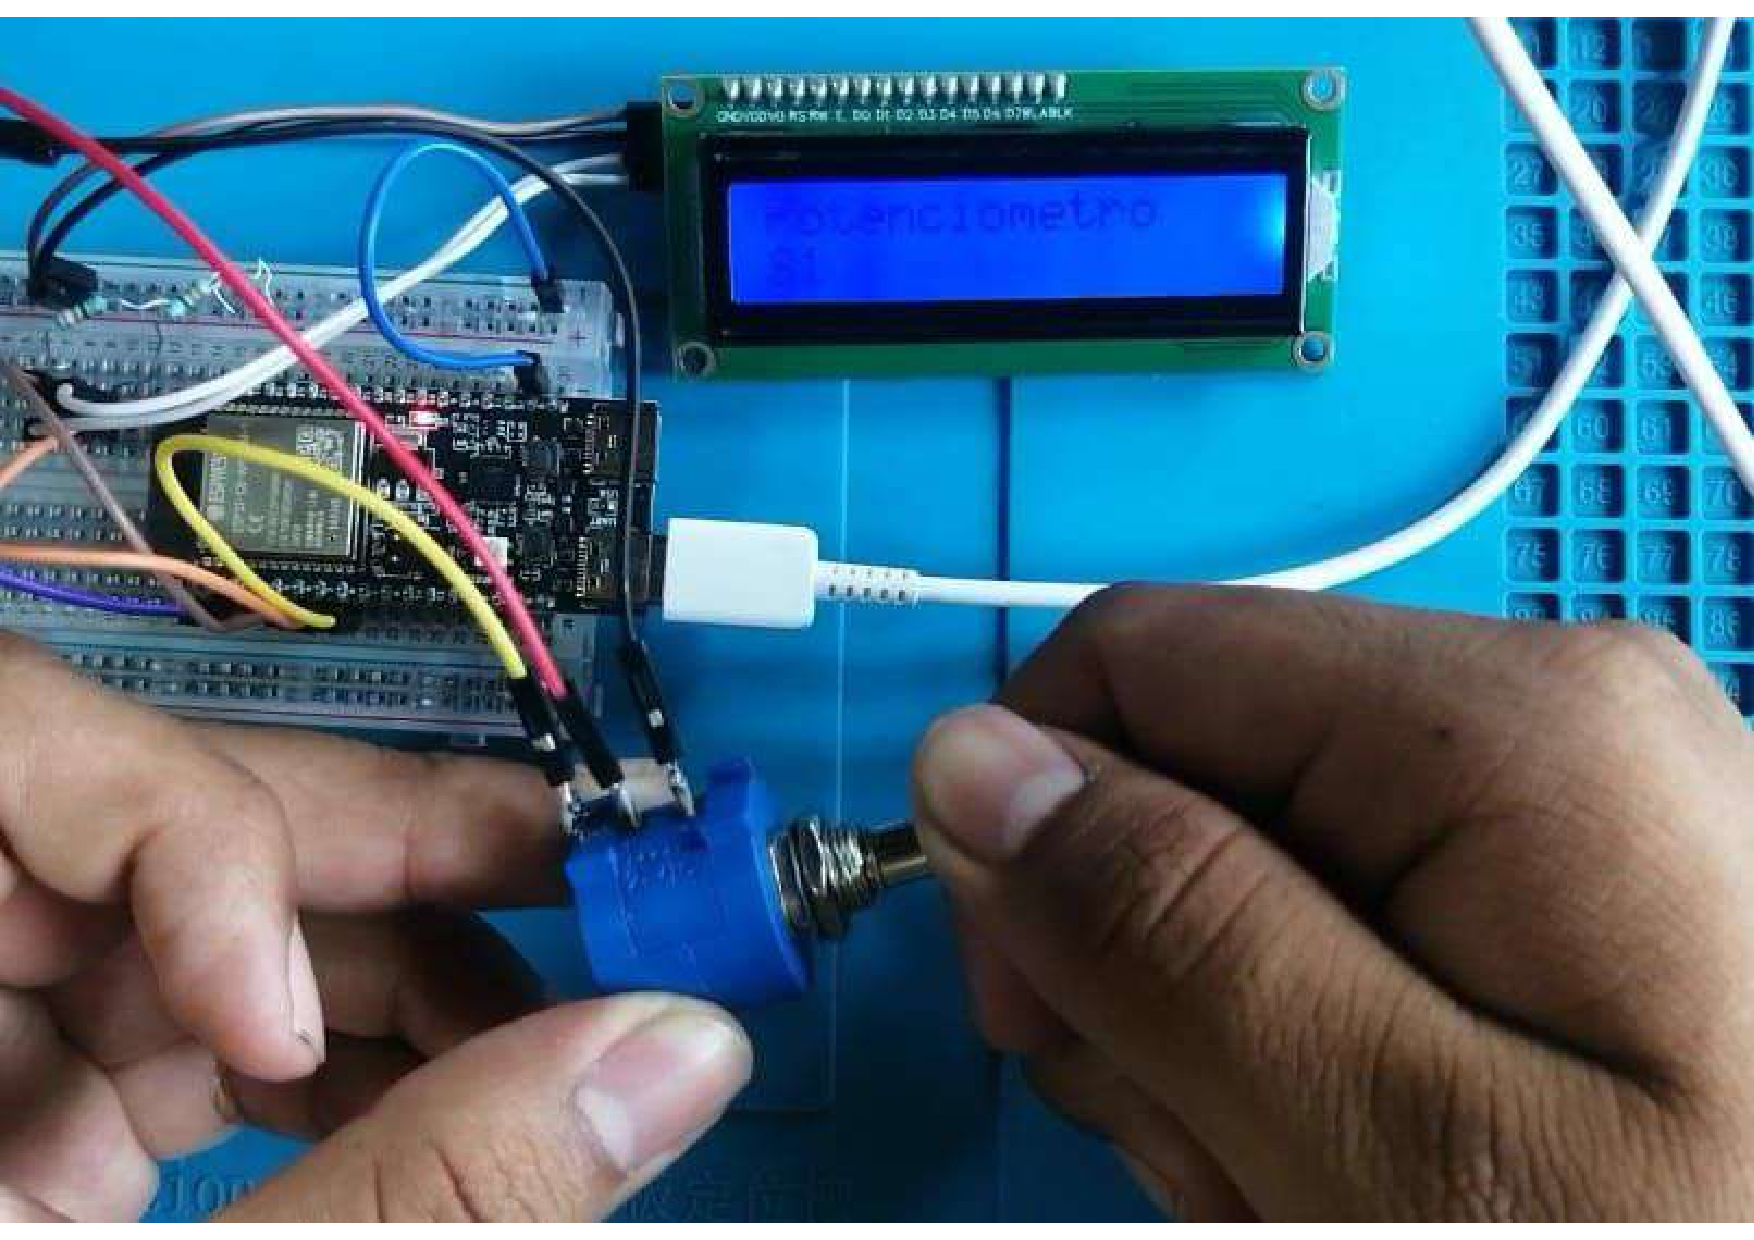
\includegraphics[trim = {45mm 15mm 80mm 20mm},clip,scale=0.5]{19/Img/evidenciaCambio6.pdf}
        \caption{Sexta lectura obtenida a la hora de armar el circuito.}
        \label{fig:evidenciaCambio6}
    \end{figure}
    Como se muestra en las figuras \ref{fig:evidenciaCambio3}, \ref{fig:evidenciaCambio4}, \ref{fig:evidenciaCambio5} y \ref{fig:evidenciaCambio6} podemos observar como estas modificaciones se llevaron acabo, pasando en un inicio de un valor de resistencia de casi 1,200 hasta llegar a uno de casi 300,sin mencionar una fluctuación en los valores al elevar y disminuir el potenciómetro, al no solo realizar una disminución en línea recta. Es decir que nuestros resultados confirman que se realizo un buen desempeño tanto del analista como del operador, ya que a pesar de haberse demorado 9 minutos en la realización del circuito este no presento ninguna falla y paso la prueba de calidad con éxito, demostrando  si bien  tanto el manual realizado como el desempeño del operador no se puede considerar el mas eficiente si se puede referir a este como exacto, al lograr el objetivo planteado de la realización del ensamble.
    
    %Antes de comenzar a preparar tu artículo, es importante que lea primero la guía del autor, la cual incluye los temas o apartados que son necesarios para tener tu trabajo completo.
    %Una vez completada la edición del texto, el documento está listo para el uso de esta plantilla. En este archivo recién creado, resalte todo el contenido e importe el archivo de texto preparado. Ahora esta listo para estilizar su documento.
    %En esta sección se deben presentar todo lo obtenido de la sección 2, incluidas deducciones o efectos del desarrollo. También se podrán incluir subsecciones numeradas de la siguiente forma:
    
    %\subsection{Autores y Afiliaciones}
    
    %Para distinguir las afiliaciones de los autores, utilice superíndices iniciando con el número 1, 2, etc., sucesivamente, esto dependerá de la cantidad de los departamentos a los que estén afiliados los autores. En caso de que todos los autores pertenezcan a una mismo departamento e institución, utilizar sólo el superíndice 1. 
    
    %\subsection{Identificar los encabezados}
    
    %Se les recuerda a los autores que los encabezados deben de estar conforme los solicita la guía del autor. De ahí se puede adaptar el trabajo para que sea más fácil de entender para el lector.
    %Los encabezados organizan los temas sobre una base relacional y jerárquica. Por ejemplo, el título del documento es encabezado del texto principal porque todo el material posterior se relaciona y elabora sobre este tema. 
    
    %\subsection{Tablas y Figuras}
    
    %\begin{enumerate}
      %  \item Posición de las tablas y figuras: Coloque las figuras y las tablas en la parte superior e inferior de las columnas. Evite colocarlos en medio. Las figuras y las tablas grandes pueden abarcar ambas columnas. Los títulos de las figuras deben de estar debajo de las mismas; los títulos de las tablas deben aparecer encima de ellas. Insértese las figuras y los cuadros después de citarse en el texto. Utilice la abreviatura “Fig. 1”, incluso al principio de una oración. 
    %\end{enumerate}
    
    \section{Conclusiones}
    
    En conclusión este método puede resultar el más sencillo y rápido de todos pero no por eso significará que perderá su validez, por lo cual aún existiendo otros métodos este es una buena opción si se posee un registro histórico con el cual comparar.
    %Se describe aquí el alcance del trabajo, logros obtenidos y perspectivas para el futuro de este. Se sugiere colocar información cuantitativa obtenida.
    
    \section{Agradecimientos}
    
    Quiero agradecer a mis compañeros los cuales se tomaron la molestia de explicarme lo básico de SolidWorks para que pudiera lograr terminar a tiempo los trabajos.
    %Es importante darles su debido reconocimiento a los laboratorios, instituciones, organizaciones, entre otros que han sido participes para la culminación de este trabajo. También es importante mencionar, fondos, proyectos, becas, entre otros que se le han otorgado al o los autores para realizar el trabajo de investigación. Ejemplo: “Los autores agradecen al Concejo Nacional de Ciencia y Tecnología por los recursos otorgados…”
    
    %\section*{Referencias}
    
    %Para esta platilla, se solicita al autor enumerar las citas de manera consecutiva entre corchetes \cite{GoA2015}. 
    %La puntuación de la oración que sigues sería \cite{RAE}. 
    %Refiérase simplemente al número de referencia, como en \cite{Morales2012}, no utilice “Ref. [3]” o “referencia [3]” excepto al principio de una oración: “La referencia [3] fue la primera…”
    %Enumere las notas al pie por separado en superíndices. Coloque la nota de pie de en la parte inferior de la columna en la que se citó. No coloque notas al pie en la lista de referencias. Utilice letras para las notas al pie de la tabla.
    %A menos de que haya tres autores o más; no utilice “et al.”. Los trabajos que no hayan sido publicados, incluso si han sido presentados para su publicación, deben ser citados como “inéditos”. Los trabajos que han sido aceptados para su publicación deben de citarse como “en prensa”. Poner en mayúscula sólo la primera palabra de un título, excepto los nombres propios y los símbolos de elemento. 
    
    % Ejemplo
    %  @Article{article,
    % 	author = "Author1 LastName1 and Author2 LastName2 and Author3 LastName3",
    % 	title = "Article Title",
    % 	volume = "30",
    % 	number = "30",
    % 	pages = "10127-10134",
    % 	year = "2013",
    % 	doi = "10.3389/fnins.2013.12345",
    % 	URL = "http://www.frontiersin.org/Journal/10.3389/fnins.2013.12345/abstract",
    % 	journal = "Frontiers in Neuroscience"
    % }
    
    % @book{book,
    %   author    = {Author Name}, 
    %   title     = {The title of the work},
    %   publisher = {The name of the publisher},
    %   address   = {The city},
    %   year      = 1993,
    % }
    
    % @incollection{chapter,
    %   author       = {Bauthor Surname}, 
    %   title        = {The title of the work},
    %   editor       = {Editor Name},
    %   booktitle    = {The title of the book},
    %   publisher    = {The name of the publisher},
    %   address      = {The city},
    %   year         = 2002,
    %   pages        = {201-213},
    % }
    
    % @InProceedings{conference,
    %   author = {Cauthor Name and Dauthor Surname and Fauthor LastName},
    %   title = {The title of the work},
    %   booktitle = {The title of the conference proceedings},
    %   year = 1996,
    %   publisher = {The name of the publisher},
    %   editor = {Editor Name1 and Editor Name2},
    %   pages = {41-50},
    % }
    
    % @book{cho,
    %   author       = {Gauthor Name1}, 
    %   title        = {The title of the work},
    %   publisher = {Country code and patent number},
    %   address      = {Patent Country},
    %   year = 2013
    % }
    
    % @book{patent,
    %   author    = {Hauthor Surname1}, 
    %   title     = {The title of the work},
    %   publisher = {Patent number},
    %   address   = {Patent country},
    %   year      = 2010,
    % }
    
    % % please use misc for datasets
    % @misc{dataset, 
    % 	author = "Author1 LastName1 and Author2 LastName2 and Author3 LastName3",
    % 	title = "Data Title",
    % 	year = "2011",
    % 	doi = "10.000/55555",
    % 	URL = "http://www.frontiersin.org/",
    % }
    
    \bibliographystyle{ieeetr}
    \bibliography{19/referencias}
    % 
    % 
    %%%%%%%%%%%%%%%%%%%%%%%%%%%%%%%%%%
    \appendix
    %%%%%%%%%%%%%%%%%%%%%%%%%%%%%%%%%%
    % 
    % 
    \centering{\section[\appendixautorefname{}]{APÉNDICE}}\label{anexo:manualOperador}
    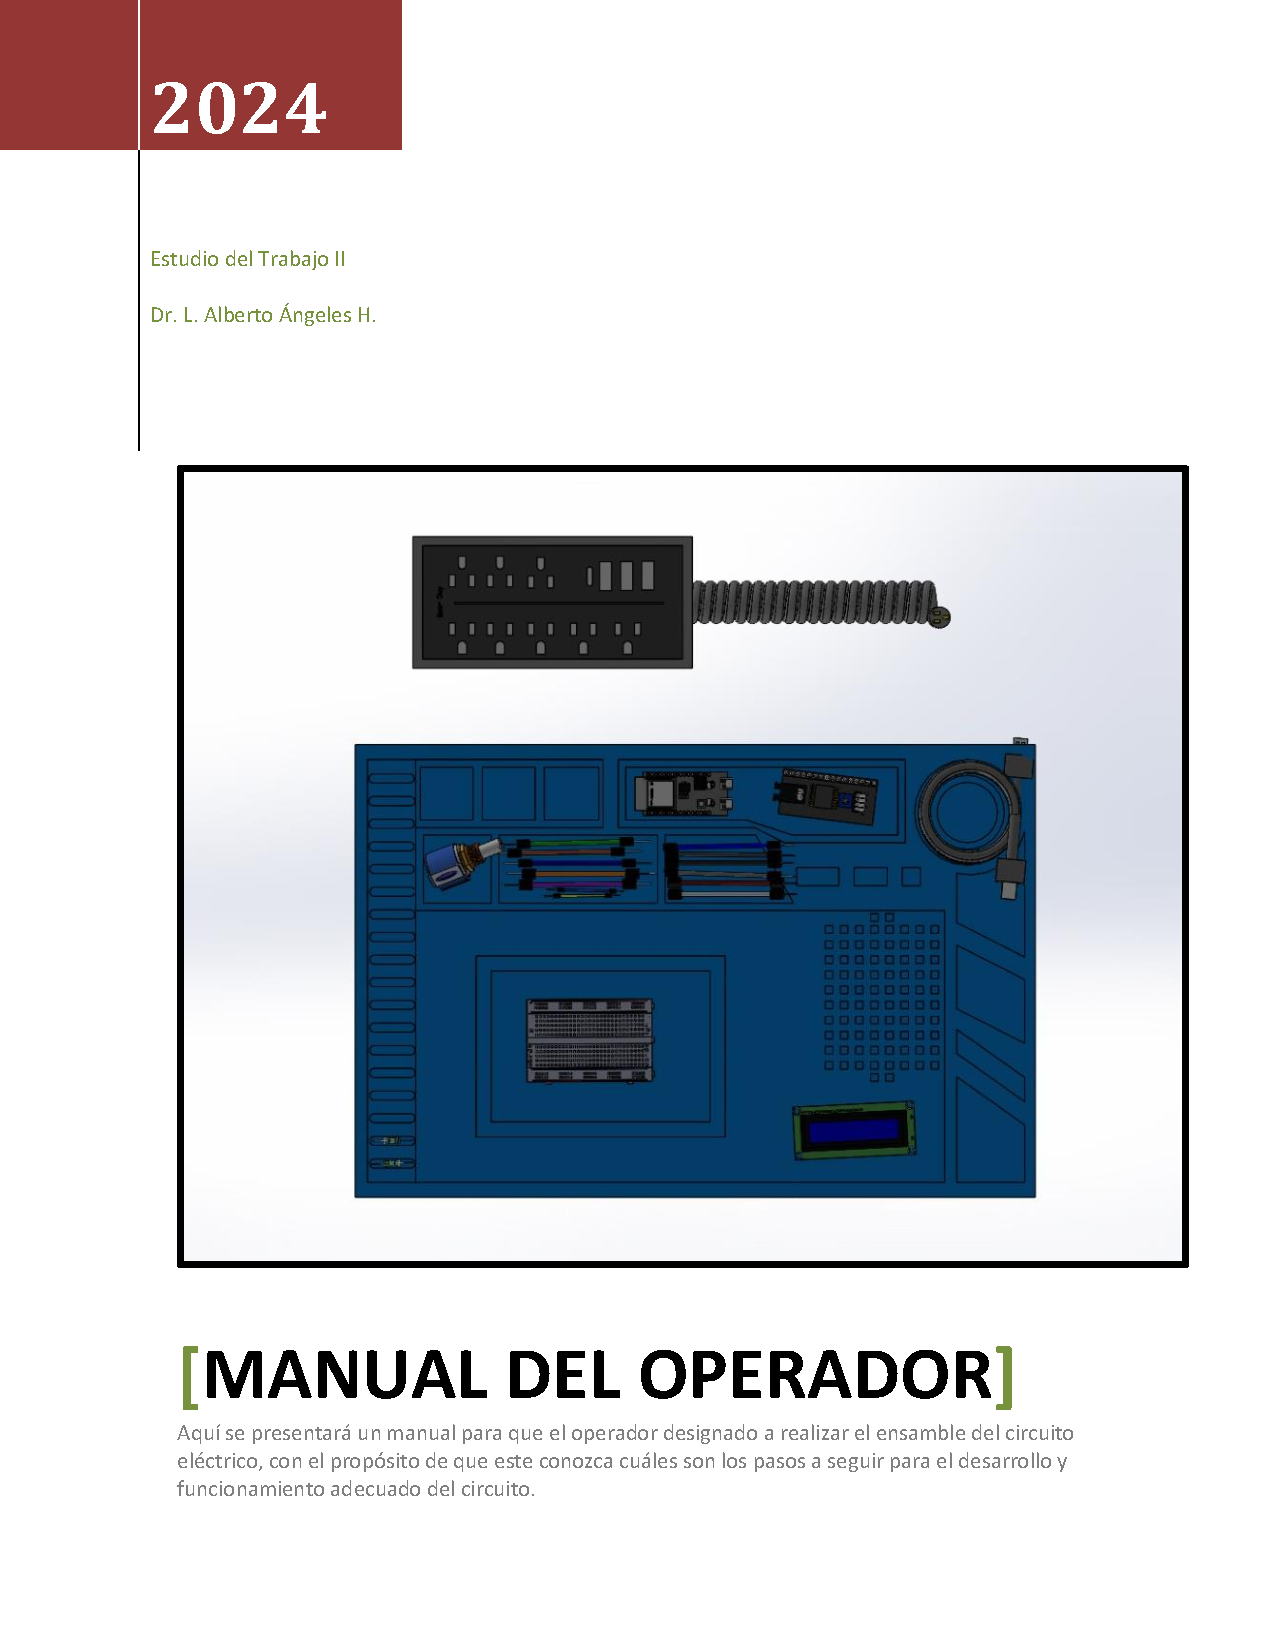
\includepdf[pages=-]{19/Img/manualOperador.pdf}
    %%%%%%%%%%%%%%%%%%%%%%%%%%%%%%%%%%%%%%%%%